%
\chapter{Spring transition}\label{ch:spring}
\section{Introduction}
The spring transition is here taken to be the period during which
the winter regime of predominant downwelling and poleward flow
over the slope is replaced by a regime of sustained coastal
upwelling. In Chapter~\ref{ch:winds} it was shown that the
transitions between regimes are largely determined by the seasonal
cycle in the meridional density gradient inferred from SST. The
first stages of this transition involve the levelling of the
poleward gradient in the sea level and are characterised by large
variability in both circulation and property distribution on the
shelf and offshore. In the absence of the steady sea level
gradient and stratification, the response of the Galician system
to upwelling favourable wind is stronger than in summer
\citet{Castro00}. During the transition, there could be short
periods during which poleward flow offshore and upwelling
nearshore coexist.

The spring transition between downwelling and upwelling regimes
can be found in all major eastern upwelling systems with a
seasonal cycle. The transition is fast in the California system
\citep{huyer83} with a time scale of few days. Equally the
response of the Galician system to upwelling winds during the
spring transition has been estimated to be fast. In other regions
like the Canary Current upwelling system, no transition is
reported though there is a lack of systematic year round
observations.

The Rias Bajas have recently started to be regarded as an
intrinsic component of the ``shelf system'' that respond to
similar forcings, i.e. large scale and local winds can drive their
circulation pattern, more so during summer when freshwater input
is at its minimum. The downwelling winds and the presence of the
poleward flow over the shelf prevents the ``outwelling'' or water
discharge from the Rias Bajas, detaining it at the inner shelf
stations \citep{Castro97} and even forcing shelfwater into the
Rias Bajas at times \citep[e.g.][]{Prego01,Sordo01}. During
upwelling winds, the Rias Bajas behave like an extension of the
shelf \citep{Doval98} and upwelling takes place inside the Rias
\citep{Alvarez-Salgado00} enhancing the flushing of the Rias.

In the next sections data from a cruise in June 1997 coincident
with the spring transition are analysed. The cruise is put into a
broader temporal context by using SST images before and after the
cruise. The sampling strategy is presented first, followed by the
data description and analysis techniques.  Horizontal and vertical
distribution of properties and velocity vectors are described next
and particular attention will be placed on the interaction of the
outflow from the Rias and the offshore circulation. The Chapter
finishes with the discussion and main conclusions.

\section{Cruise description}
The RRS Charles Darwin Cruise 105 took place in the Galician CTZ
from 29 May to 20 June 1997 as part of the OMEX II-II project. The
cruise was divided into two legs: leg A ran from 29 May to 8 June
while leg B ran from 10 to 20 June. The main objectives of the
cruise were:

\begin{itemize}
  \item  to make a detailed swath bathymetry of the slope topography of the
  region during leg A.
  \item  to deploy a
bottom-mounted acoustic Doppler current profiler at 156m depth and
a mooring of four current meter in 686m, both near 42\deg 40'N,
  \item to sample a grid of CTD stations typically 10km apart on
  cross slope sections ranging from 43\deg N to 41\deg 25' every 10' of latitude
  and covering depths from 100m on the shelf to 3000m offshore,
  \item to record underway ADCP, temperature, salinity,
  fluorescence, transmittance and irradiance.
\end{itemize}
The sampling of the slope bottom topography was carried out during
leg A and only underway Temperature and Salinity were recorded for
that period. The CTD grid sampling took place during leg B. The
grid stations were roughly separated 10 by 18 km, smaller than the
local internal Rossby radius of 20-30km \citep{Chelton98} which
provided enough detail to resolve mesoscale structures. However,
the 10 days it took to complete the survey compromised its
synopticity. Besides the standard CTD measurements of temperature,
salinity and pressure, the instrument was also equipped with a
fluorescence sensor.

Downwelling favourable wind conditions were typical for the first
4 days of Leg B with increasing northerly winds thereafter until
the end of the cruise on 20 June. The moorings were deployed on
the first day (10 June) and the CTD grid started on the following
day. The 3 northernmost grid lines (Transects N,O and P,
Fig~\ref{fig:cd105stations}) were done first during downwelling
wind conditions, while the remainder of the grid was completed
northwards from the southern most deep station in the order V-Q
under upwelling conditions.
\section{Data and Methods}
\subsection{CTD}
A total of 82 CTD stations were sampled with a Neil Brown Systems
Mk IIIB CTD including a pressure sensor, a conductivity cell, a
platinum resistance thermometer and a Beckmann dissolved oxygen
sensor. The CTD unit was mounted vertically in the centre of a
protective cage approximately 1.5m square. A Chelsea Instruments
Aquatracka configured as a fluorometer was also attached to the
system.

A General Oceanics 12-bottle tone-fire rosette pylon was fitted to
the top of the CTD frame. 10-litre Niskin bottles were used
throughout the cruise.

On each cast, the CTD was lowered continuously at 0.5 to 1.0\vel\,
to about 20-30m from the sea floor. The data were logged by the
NERC Research Vessel Services (RVS) ABC data logging system.
Output channels from the deck unit were logged at 32 Hz by a
microprocessor interface (the Level A) which passed time-stamped
averaged cycles at 1 Hz to a Sun workstation (the Level C) via a
buffering system (the Level B).
\begin{figure} \centering
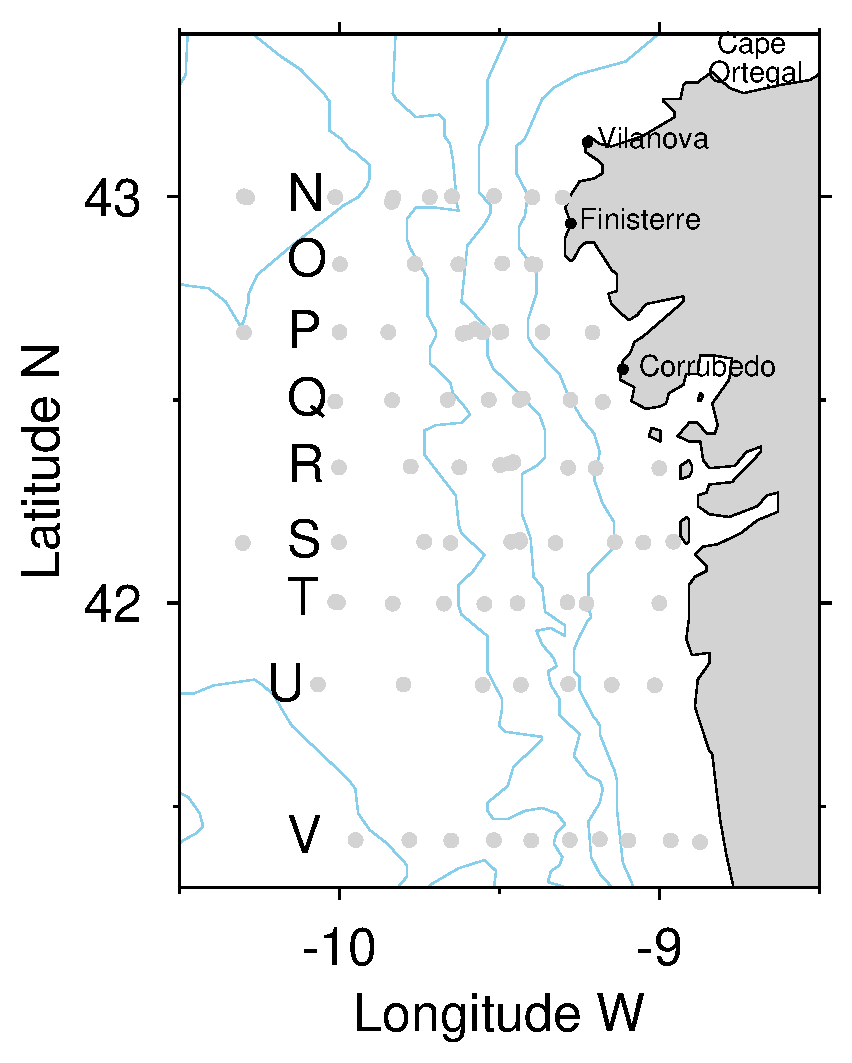
\includegraphics[width=7cm]{cd105stations}
\caption{Location of Coastal weather and CTD stations and Transect
names for CD105 cruise} \label{fig:cd105stations}
\end{figure}

The data were subsequently transferred to the British
Oceanographic Data Centre (BODC) where it was converted to
specific BODC data format. The data were separated into downcast
and upcast and edited for spikes or spurious data. The downcasts
were logged into the BODC system, calibrated and binned to 2dbar
prior to their release to the OMEX II community.

The temperature sensor was calibrated against on board
measurements from a digital reversing thermometer at depths
greater than 1000m. Agreement was found within the manufacturers
specifications and no correction was applied.

The salinity sensor was calibrated against 47 bottle samples
analysed on a Guildline Autosal bench salinometer and a constant
offset of 0.024psu ($\pm$0.005psu) was applied.

\subsection{Underway measurements}

The ship was fitted with a non-toxic pumped sea water supply with
water drawn from an inlet approximately 5m below the surface,
amidships on the starboard side. All ship's discharges were to
port to minimise risk of contamination. Water from the non-toxic
pump was fed into the thermosalinograph and the tank containing
the fluorometer and transmissometer.

Continuous data from the Falmouth Scientific Instruments
thermosalinograph were recorded every minute during both legs of
the cruise. During leg A only Temperature and Salinity were
recorded. In leg B,  chlorophyll data were measured by a Chelsea
Instruments Aquatracka fluorometer.

Where possible, data collected from underway sensors were
calibrated against CTD data and/or discrete samples from the
non-toxic supply or CTD rosette bottles. A constant offset of
-0.024\deg C (N=77,$\pm$0.0305\deg C) and -0.081psu
(N=85,$\pm$0.0109psu) were found for the temperature and salinity
sensors.

The data were also logged by the RVS ABC data logging system as
were the position data from GPS, primarily an Ashtech 3-D GPS
system.

\subsection{ADCP data collection and calibration}
\subsubsection{Instrumentation and acquisition}
A RDI Acoustic Doppler Profiler (ADCP) 150 kHz instrument was used
during the cruise.  The ADCP transducer transmitted sound pulses
every few seconds in four separate beams. Each beam was oriented
at a 30 degree angle from the ship's vertical axis. The transducer
was mounted roughly amidships at 5m below the water. The data
acquisition system consisted of an IBM-PC compatible computer
running the  RDI TRANSECT program. The navigational data and the
ADCP raw data were merged at the RVS ABC system level C. The
instrument was set up with a pulse length of 4m, a band width of
4m, a blanking interval of 4m, and an ensemble averaging of 5min.
The number of processed and recorded bins had been set to 100,
about twice the actual number of good bins. Because of the
additional processing time, the number of pings per ensemble was
greatly reduced and the quality of the final data set degraded.
The error velocity threshold for raw pings during acquisition was
1\vel\, and bins with less than 25\% of percentage good (PG) were
automatically flagged. No correction for pitch and roll were made;
errors associated with these are likely to be small
\cite{kosro85}. The data were recorded continuously from 10 June
08:39 to 20 June 16:47.
\begin{figure}[tbh]
  \centering
  \begin{minipage}{7cm}
  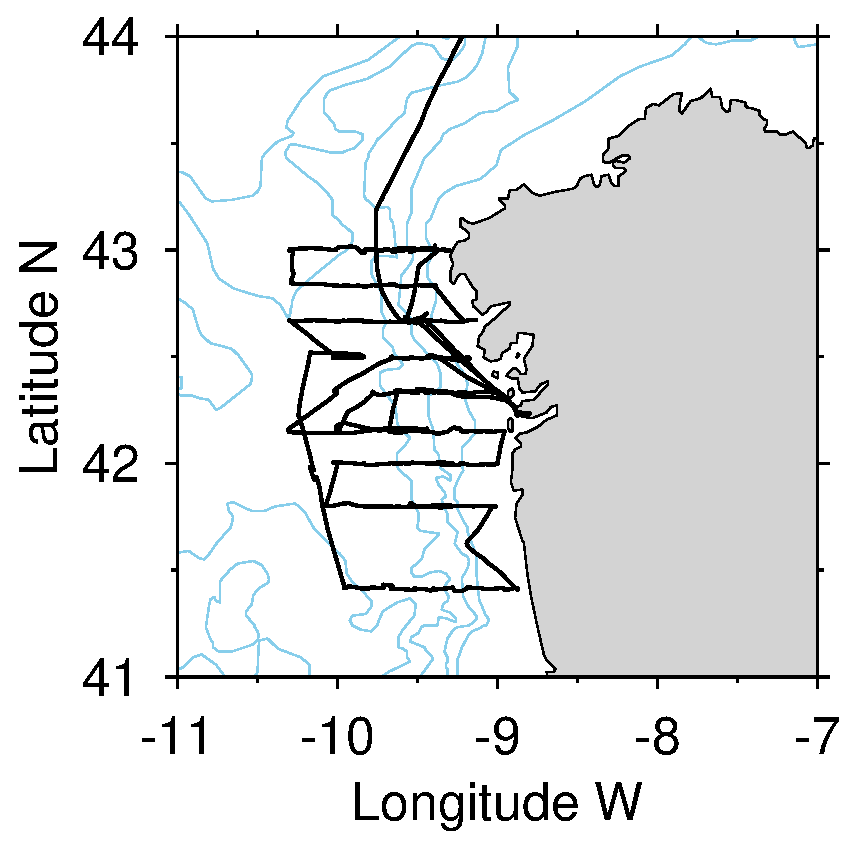
\includegraphics[viewport=0 0 400 400,width=6.8cm,clip]{cd105adcptrack}
  \end{minipage}
  \begin{minipage}{7cm}
  \includegraphics[viewport=20 40 430 260,width=7.8cm,clip]{cd105lat}
  \includegraphics[viewport=17 40 430 260,width=7.8cm,clip]{cd105lon}
  \end{minipage}
  \caption{Cruise track and longitude and latitude displacement from ADCP during
   CD105 cruise}
  \label{fig:cd105track}
\end{figure}
The sampling track and the longitude and latitude time series
estimated from the edited GPS record are shown in
Fig~\ref{fig:cd105track}. The Percentage-good (PG) pings against
time and depth (bin number) during CD105 decreased towards the
bottom (Fig~\ref{fig:cd105pg}, darker colours indicate lower PG).
The black region of low PG can generally be related to
interference with the seafloor. The echo intensity from a hard
surface such as the bottom is much stronger than the echo from
scatterers in the water and for an ADCP with 30\deg beam angle,
the echo from the side lobes facing the bottom will return to the
ADCP at the same time as the echo from the main lobe at 85\% of
the distance to the bottom. This means that data from the last
15\% are usually contaminated and were therefore removed. The bulk
of the water column recorded values higher than 80\%, however the
first 1-2 bins appeared contaminated with values between 40-80\%
and were carefully inspected and dropped when necessary. The last
good record that had been used for plotting later in the chapter
was on 20 June 07:12 after which data degraded considerably due to
worsening of weather conditions.
\begin{figure}
  \centering
  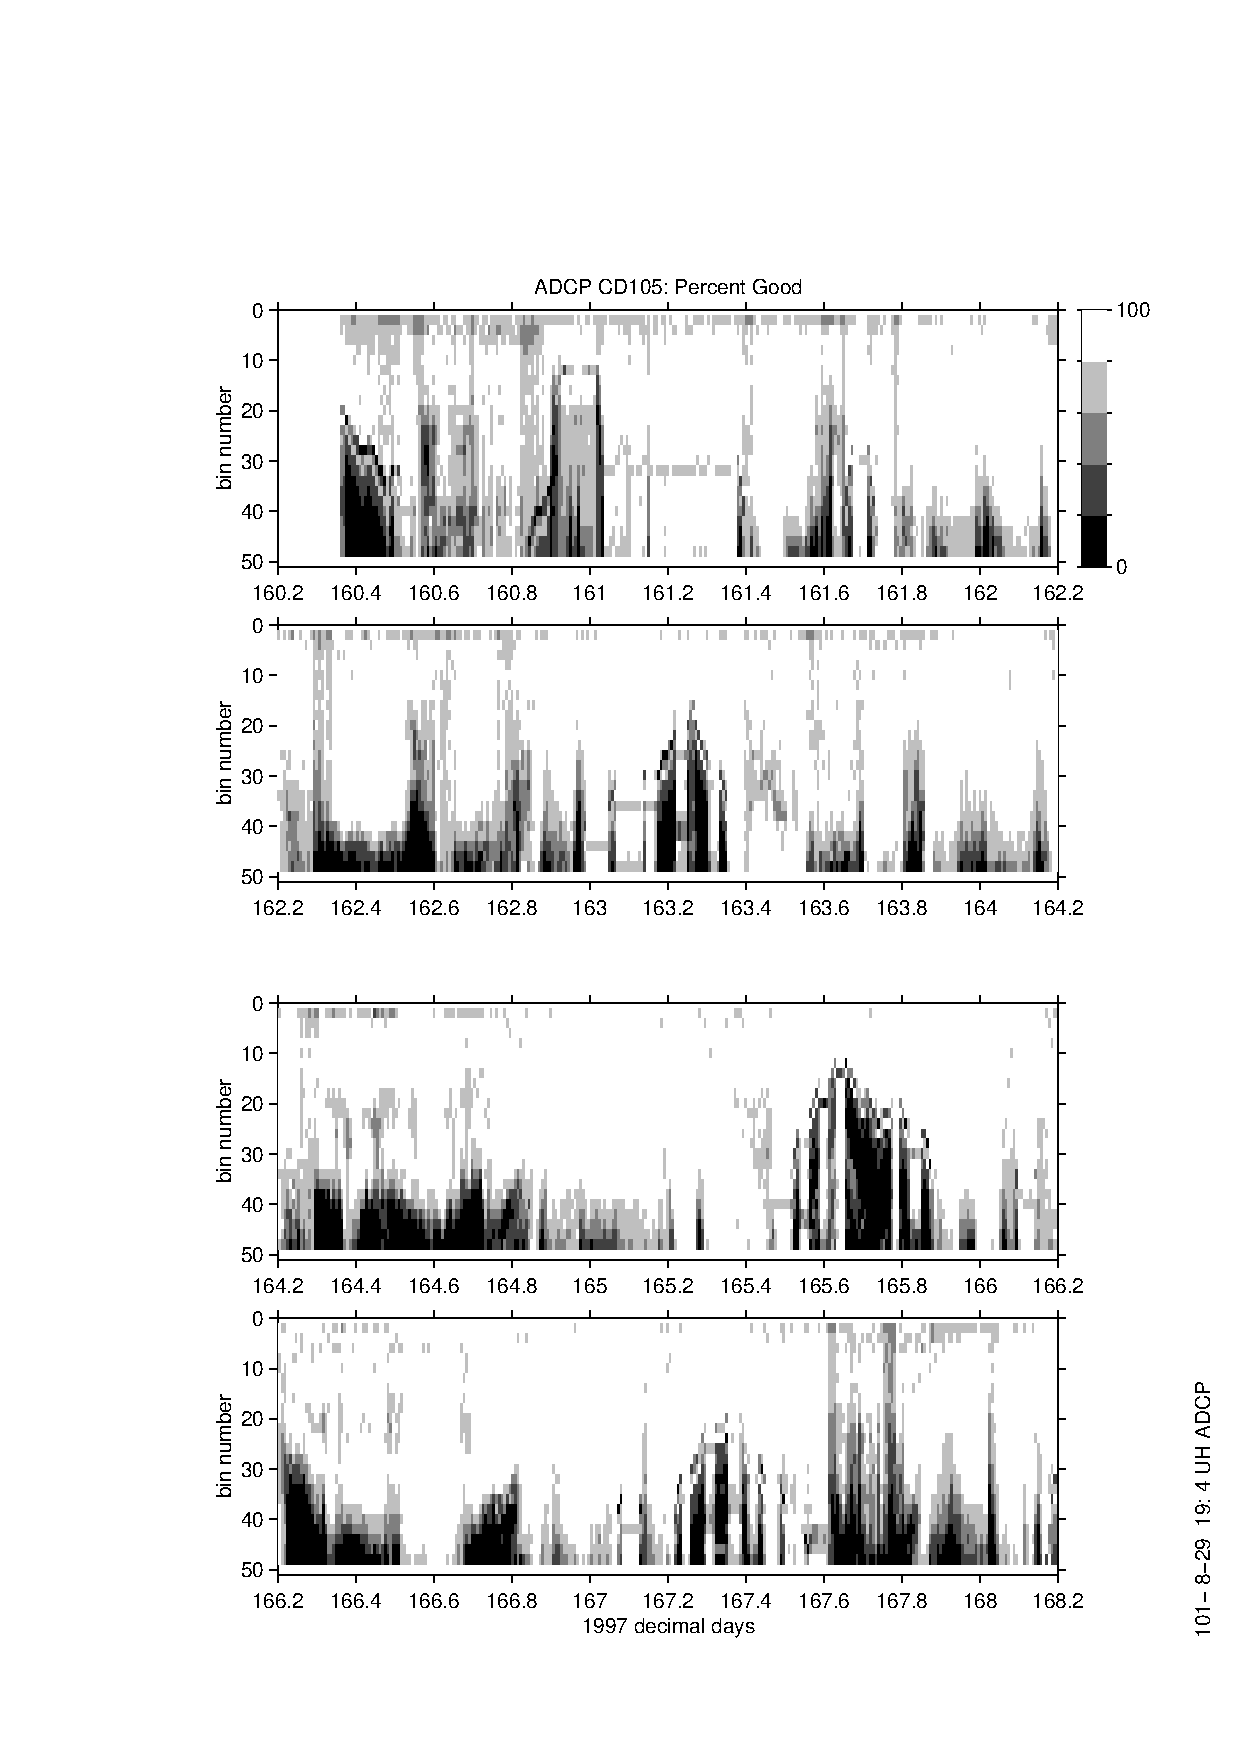
\includegraphics[viewport=0 0 460 700,width=8.5cm,clip]{pgood160}
  \caption{Percentage-good pings vs. time and bin number during CD105}
  \addtocounter{figure}{-1}
  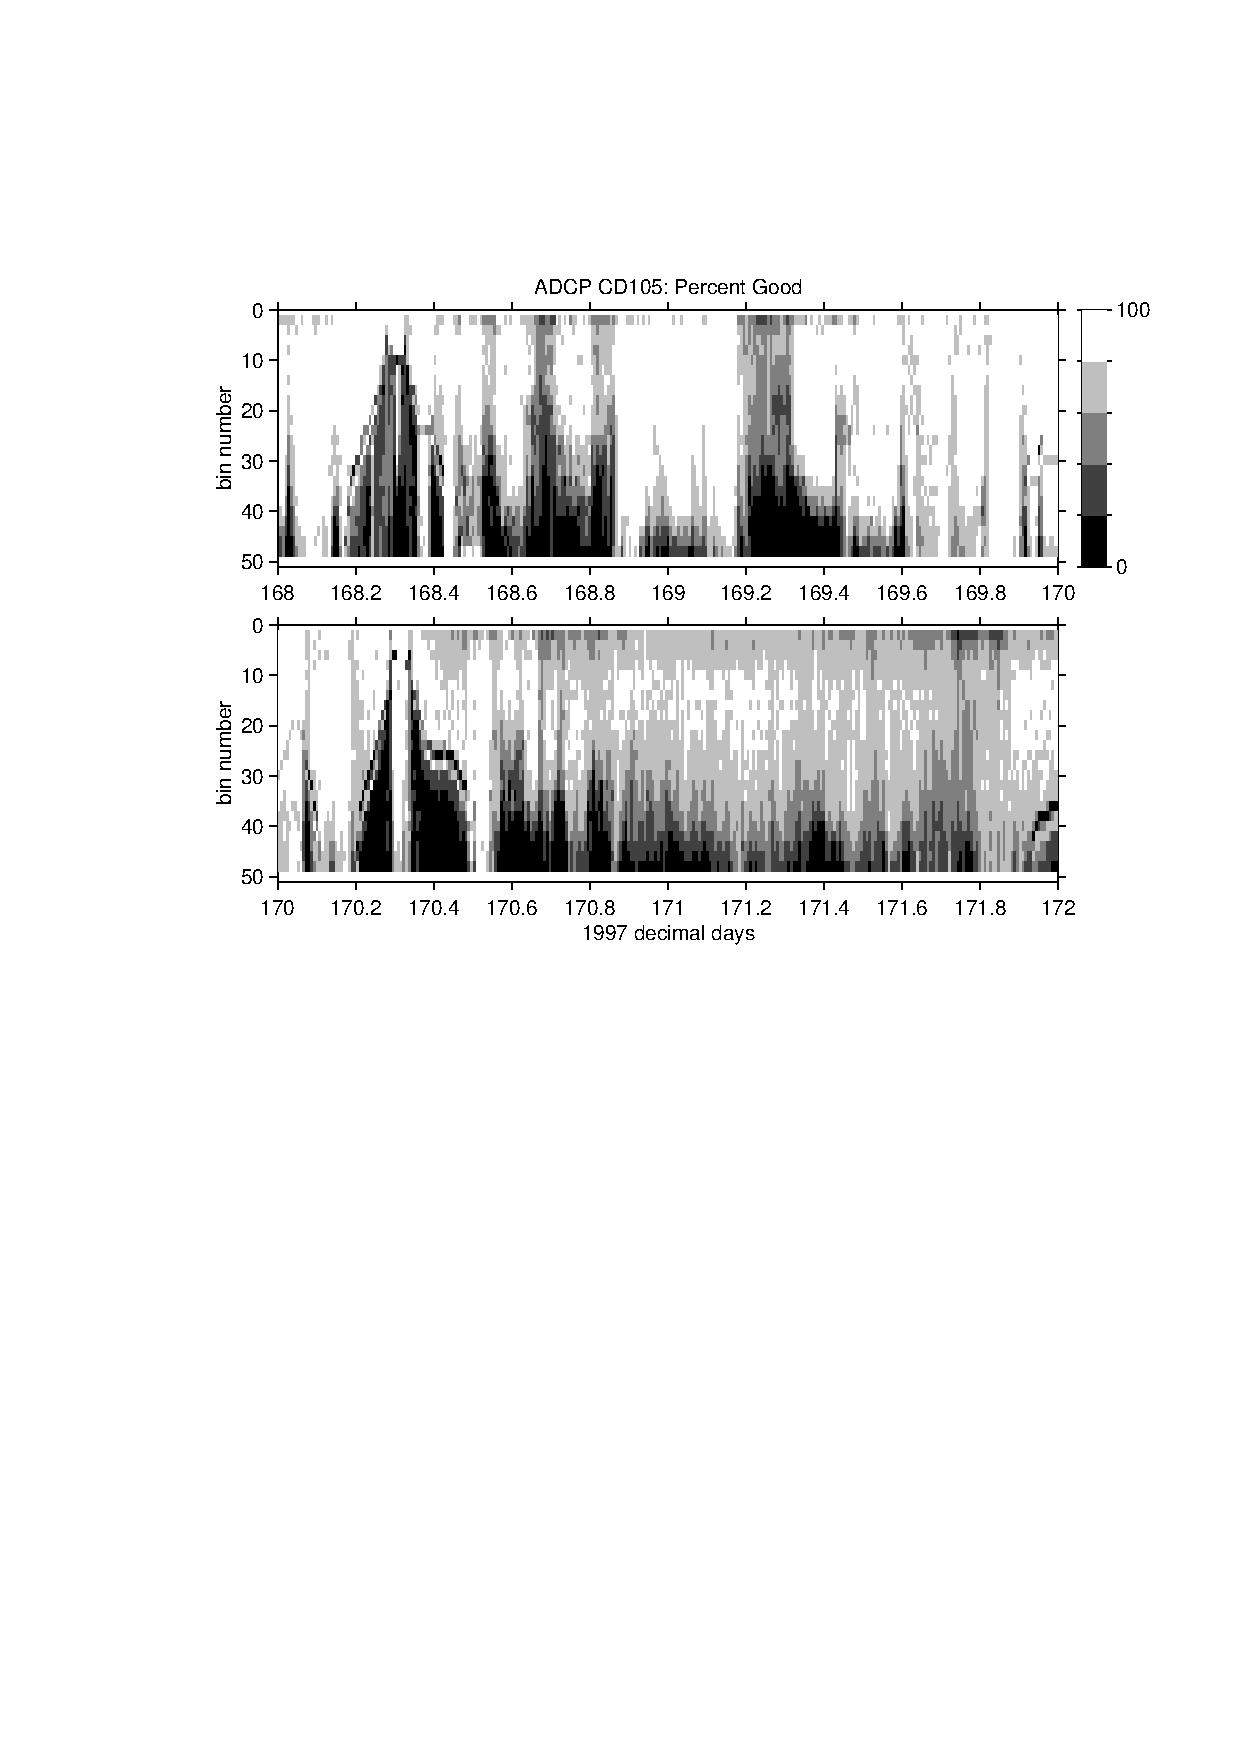
\includegraphics[width=8.5cm]{pgood168}
  \caption{Percentage-good pings vs. time and bin number during CD105, cont.}
  \label{fig:cd105pg}
\end{figure}

\subsubsection{ADCP data processing}
ADCP processing was done with the Common Oceanographic Data Access
System (CODAS), which includes MATLAB routines, developed at the
University of Hawaii by Eric Firing and Ramon Cabrera with
subsequent updates by Julie Ranada \citep{codas}. The system
consists of several iterative programs to carry out editing,
calibration, navigational correction and plotting of the ADCP
database.
%\begin{figure}
%  \centering
%%  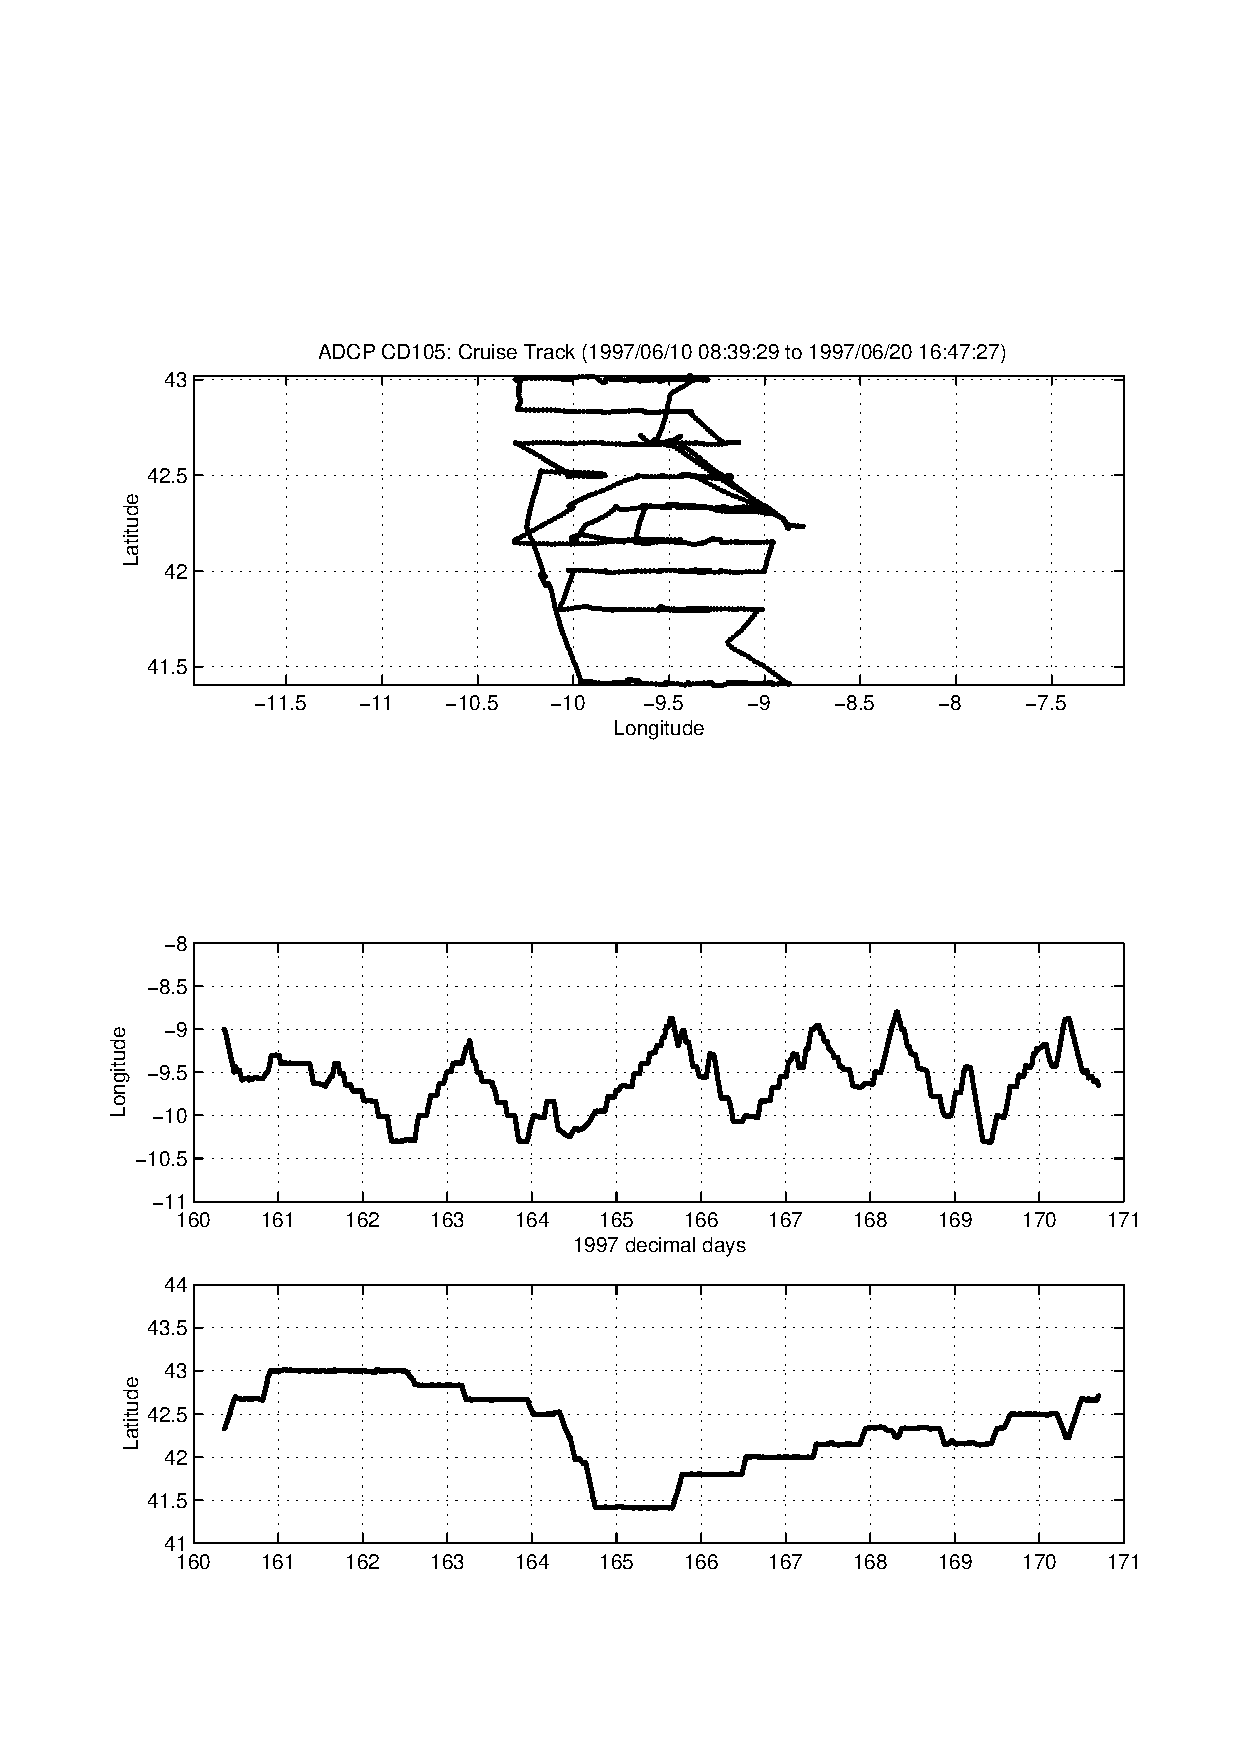
\includegraphics[viewport=0 0 553 400,width=9cm,clip]{./graphics/cruistrk}
%  \caption{Codas processing diagram}\label{fig:codasdiag}
%\end{figure}
%
\paragraph{Editing}
The principal objectives of the editing stage are to identify when
and at what depth the acoustic beams reflect off the bottom (in
shallow water), to set the top bin at which a profile contains
good data, and to flag bins contaminated by interference from
physical objects, such as the winch wire during a CTD cast, or by
other random occurrences such as instrument failure. The main
editing steps are:

\begin{itemize}
  \item Set thresholds for the quality control test. These are
  specific to the data set and depend upon some basic statistics
  from the cruise long record. First the error velocity is used
  which comes from the redundancy in the 3-dimensional velocity
  estimates \emph{u,v,w} and allows the four beam RDI system to calculate two
  different estimates of the vertical velocity. Large
  discrepancies between the two indicates an inconsistency among
  the oceanic velocities sampled by each beam. Individual bins
  with an error velocity larger than 14\velc\, were rejected. Other
  quality parameters used were the second differences with respect to
  depth of the horizontal (\emph{d2uv}) and vertical (\emph{d2w}) velocities
  for each profile. If \emph{d2uv} or \emph{d2w} exceeded
  global 2 standard deviation thresholds, the bin was rejected.
  Entire profiles were also flagged if the standard deviation of
  \emph{w} exceeded a global 3 standard deviation threshold.
  \item Employ the CODAS/MATLAB editing system to view various
parameters such as relative velocities, return signal amplitude,
error velocity and percentage good. At this stage the quality
thresholds from above were applied and careful inspection of each
individual profile determined whether the automatic flagging was
accepted. The signal from the bottom was determined by jumps in
the Automatic Gain Control (AGC, which gives an indication of the
echo return signal strength; 1AGC count correspond to about 0.45dB
change in signal power) larger than 20. The deepest subsequent bin
was taken as the bottom depth and 15\% of the profile depth was
flagged to account for interference from the reflected signal.
\item Reject or accept the flagged bins and profiles which are
automatically placed in output files based on the type of error.
\item Update the ADCP database by setting the maximum depth
(bottom), setting  the top good bin, and flagging suspicious bins
for each of the profiles.
\end{itemize}
An indication of the data set quality can be inferred by looking
at cruise-long averages of key variables like the PG, AGC and
error velocity profiles at both underway (UW) and in station (ST)
shown in Fig~\ref{fig:cd105qual}. The variables were plotted to
the maximum depth of usable data, 200m, below which no ADCP data
will be discussed. From the set of variables, some indicate a
certain degradation in the data quality while underway like the PG
and Error velocity. The return signal amplitude was larger at
shallow depths as expected, gradually decreasing with depth, never
reaching a constant noise level. No significant differences can be
observed between ST and UW data in either the mean or standard
deviation statistics. The PG mean profiles showed the same shape
with depth in ST and UW data, however UW recorded values smaller
by 10-20\%. Overall, no bins recorded 100\% of PG, with the
maximum 85-90\% (70\%) in ST (UW) data situated around 40m and
decreasing either side. The PG threshold for `good data' was set
to 30\% which corresponds to 175m (160m) in ST (UW) records. The
low PG return at the shallowest bins might be related to the
physical installation of the ADCP transducer in the Charles Darwin
and similar problems were experienced in a later cruise on the
same ship (see Chapter \ref{ch:summer}). The mean vertical
difference of the horizontal components of velocity were
relatively small over the depth range, generally less than
2.5\velc, but very variable. However no significant changes were
noticeable between ST and UW data. Nonetheless, the spikiness of
the profiles suggest that a larger vertical averaging is required
in order to reduce the variability and indeed the ADCP data later
shown in the chapter corresponds to 10m or larger vertical means
and at least 10min temporal averages. Vertical velocity values
were relatively small as expected and discrepancies between ST and
UW profiles were restricted to the shallowest bins. The larger
values found below 160m are another indication of decreased data
quality. The Error velocity profiles showed the largest and more
consistent differences between ST and UW data. Maximum values of
0.2\velc\, were measured while in station while values of 1\velc\,
were typical of UW profiles.

\begin{figure}[t]
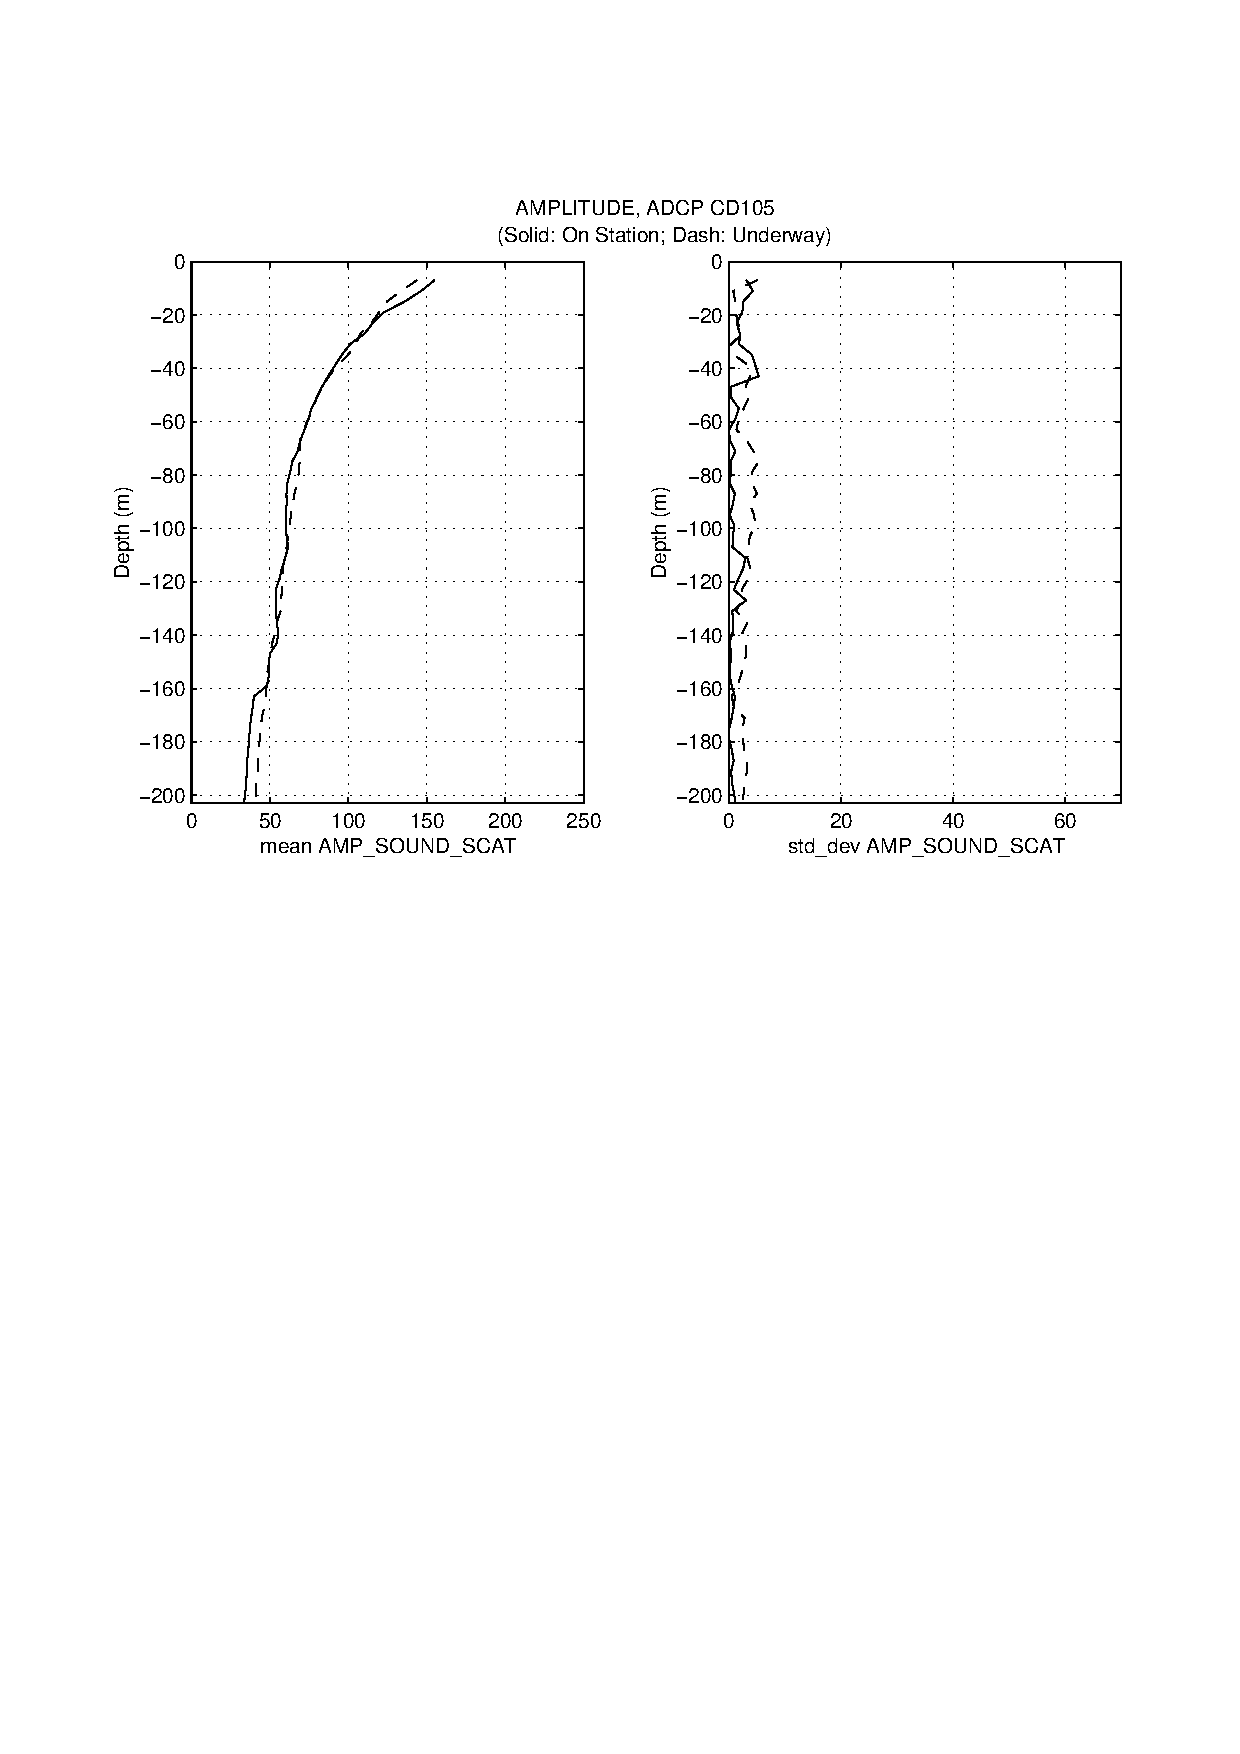
\includegraphics[width=7cm]{quality_A}%
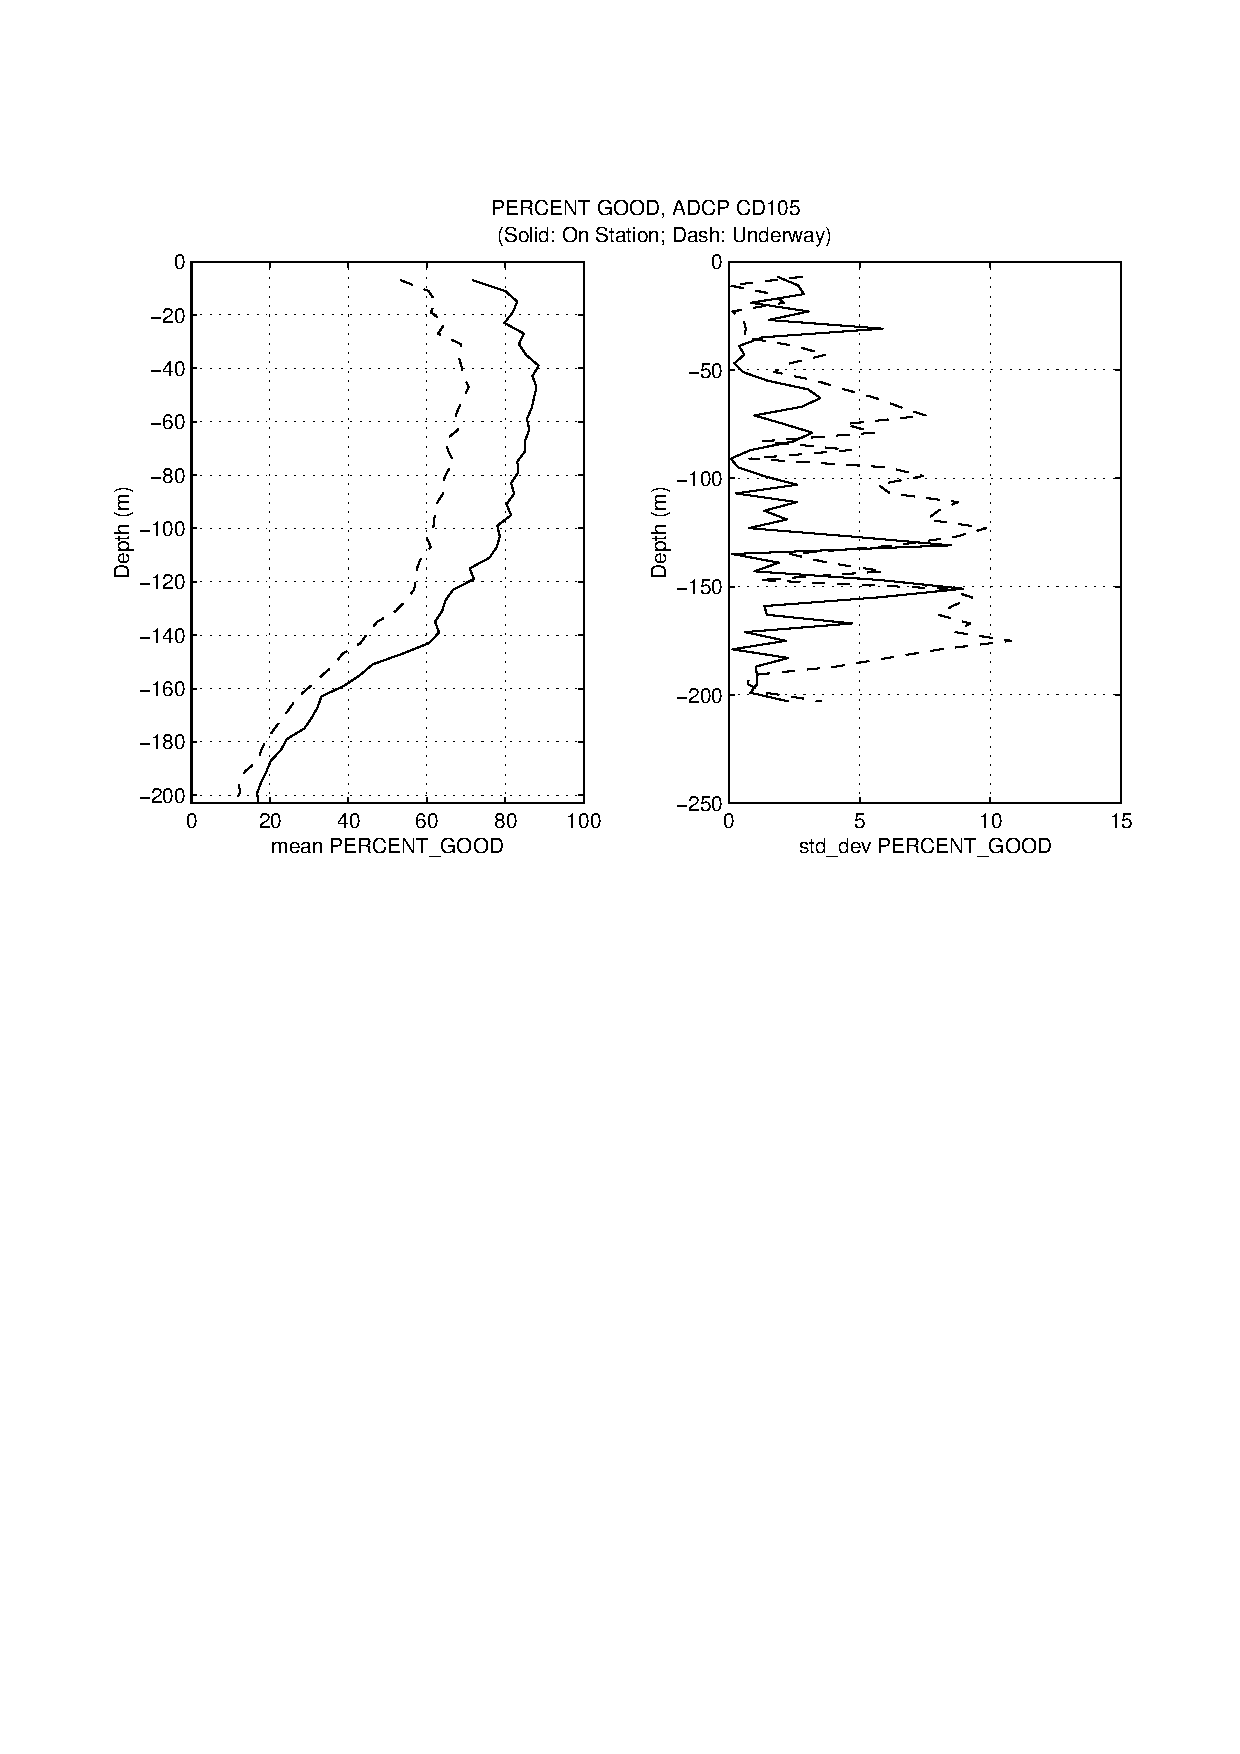
\includegraphics[width=7cm]{quality_P}
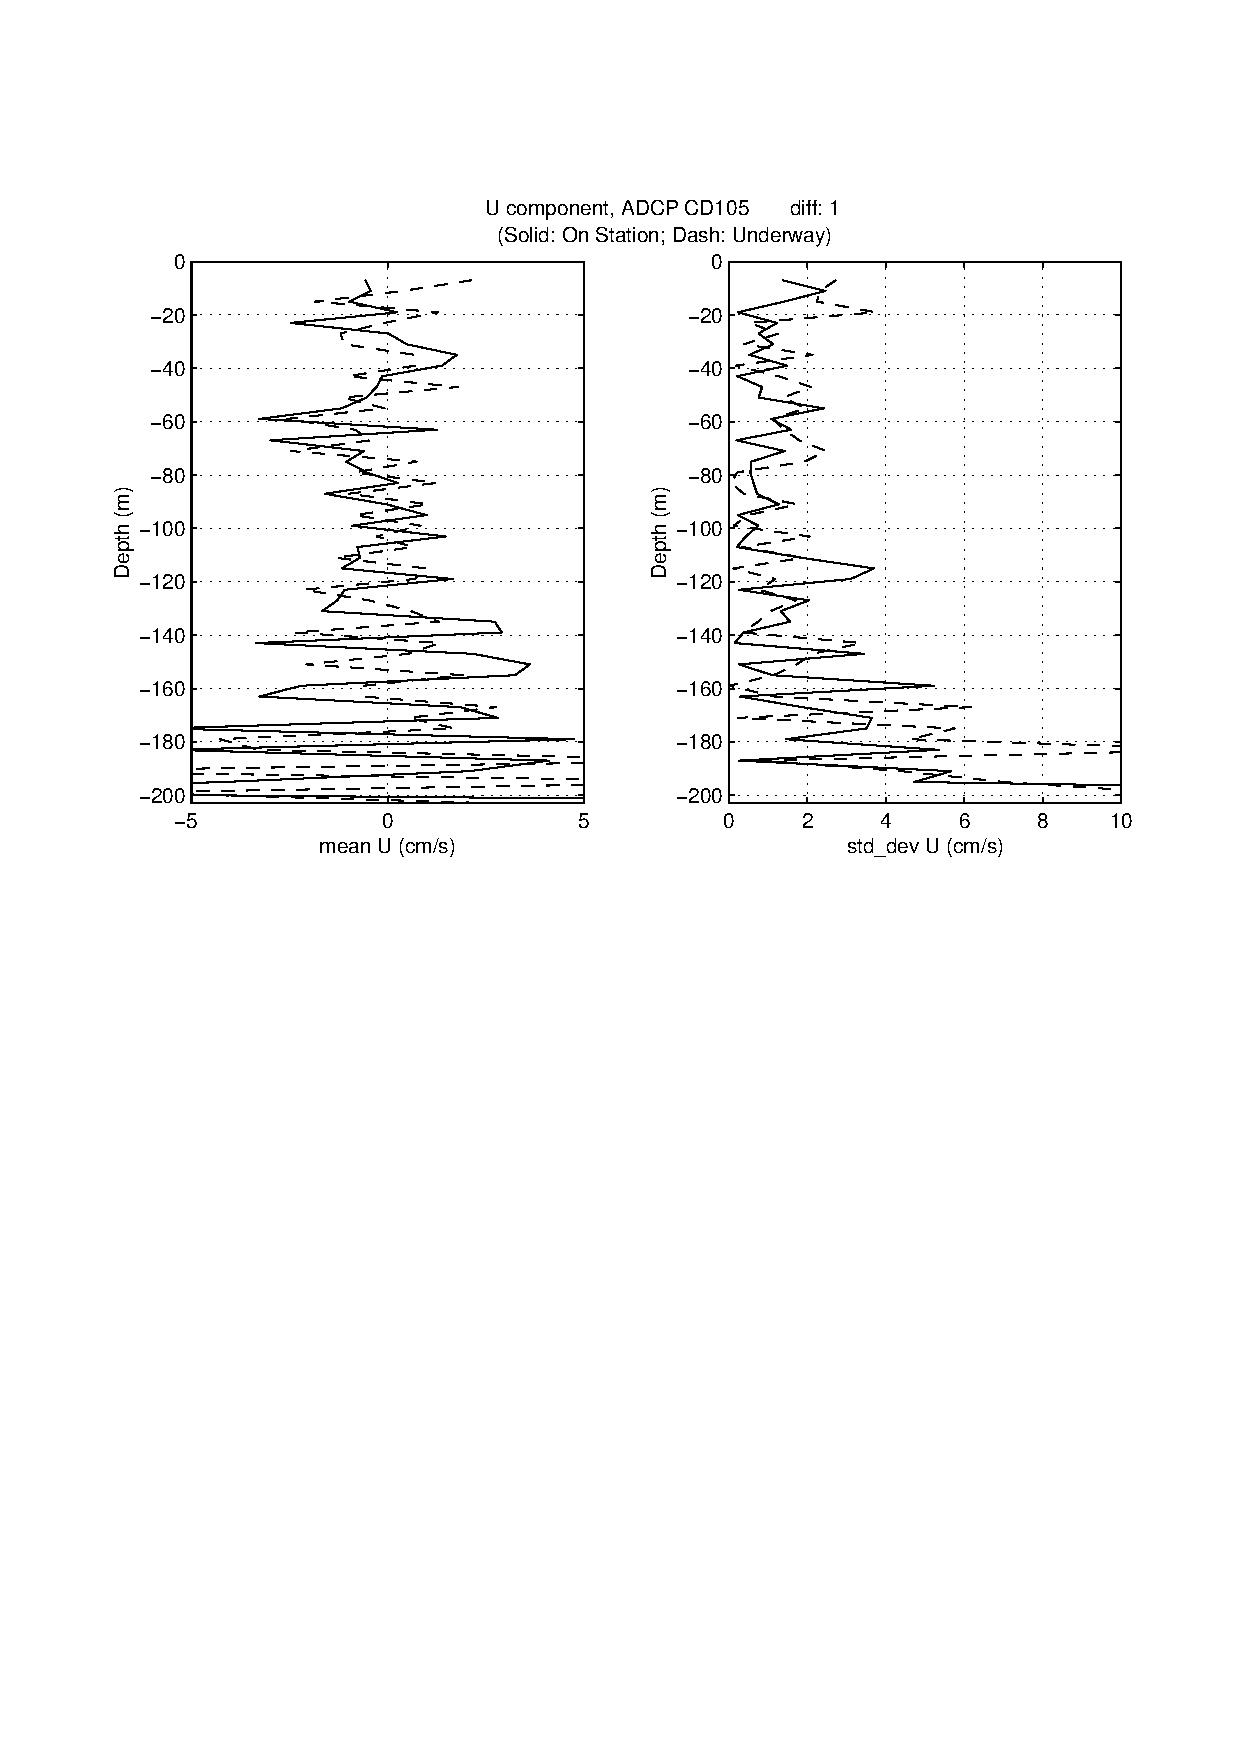
\includegraphics[width=7cm]{quality_U}%
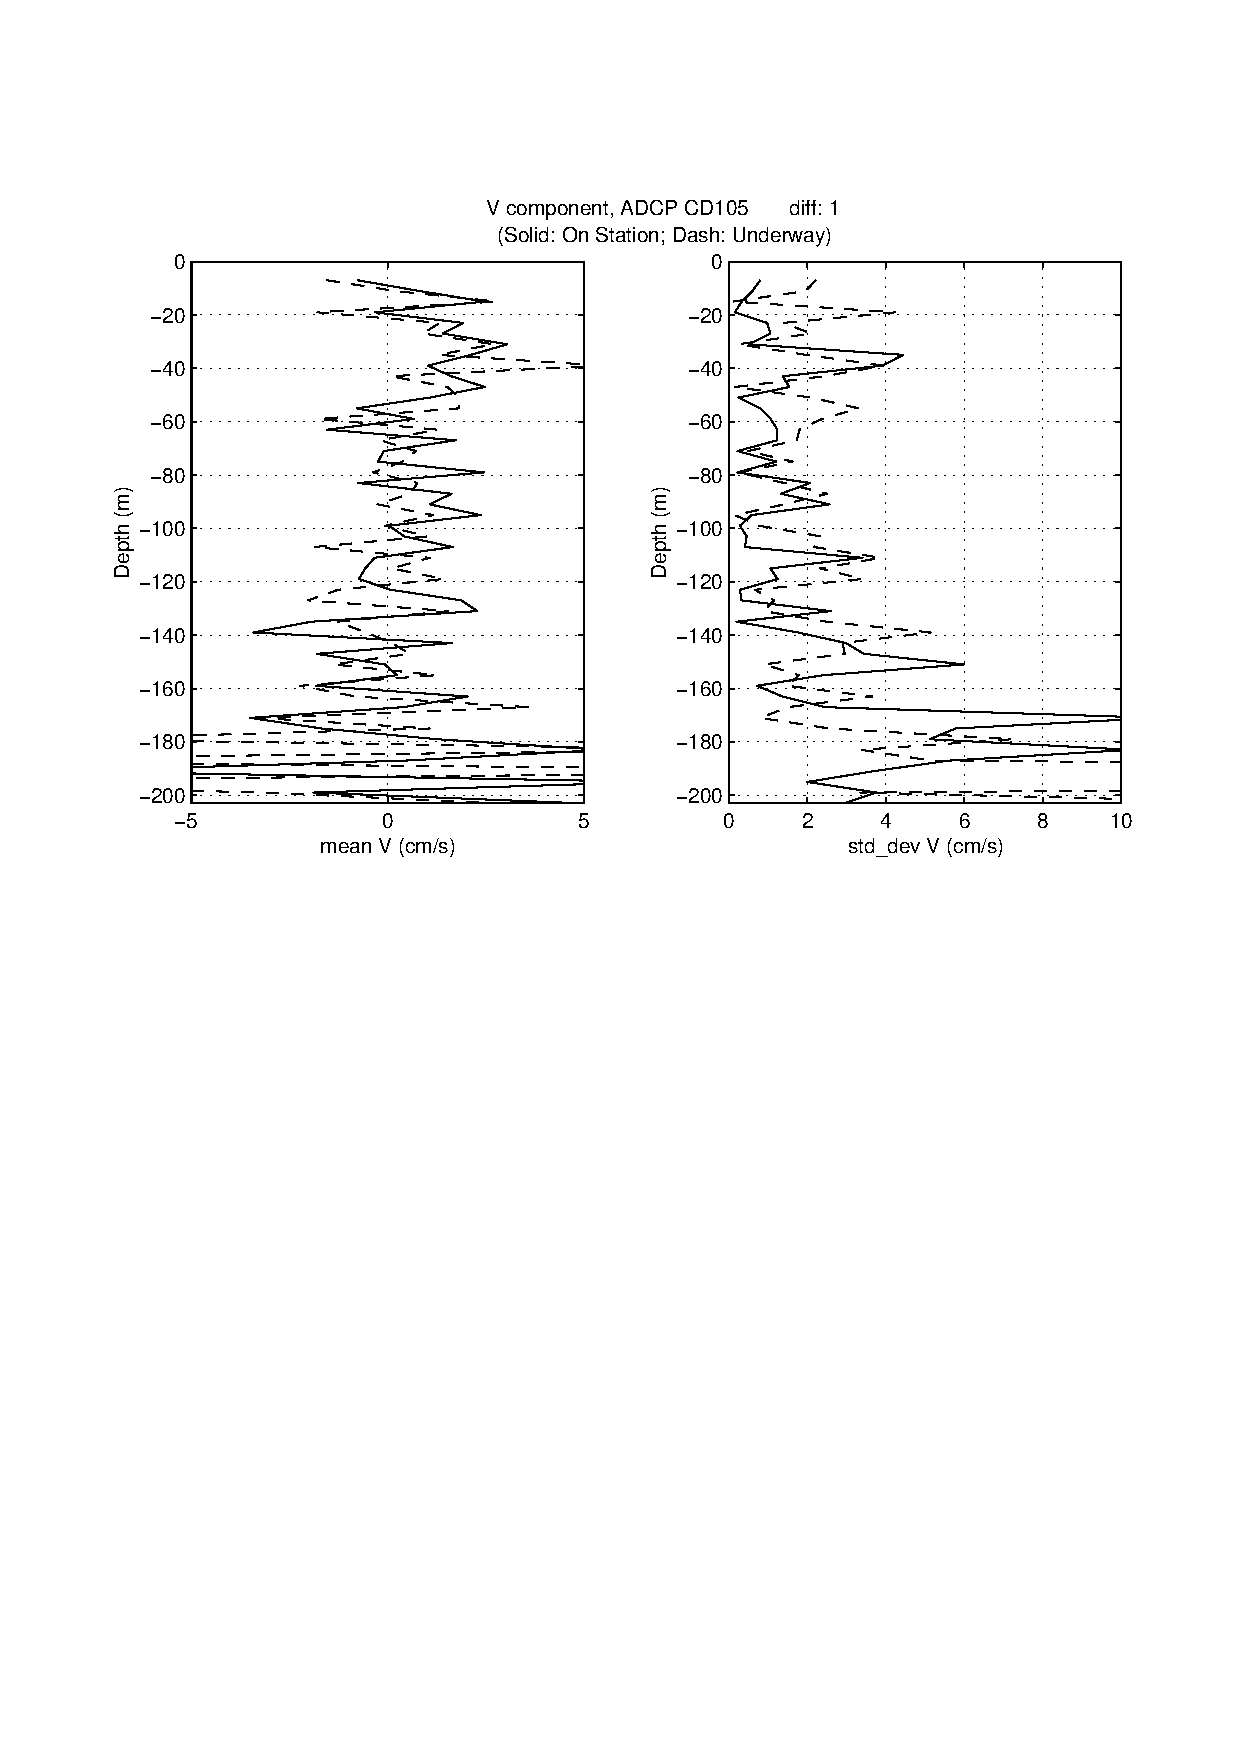
\includegraphics[width=7cm]{quality_V}
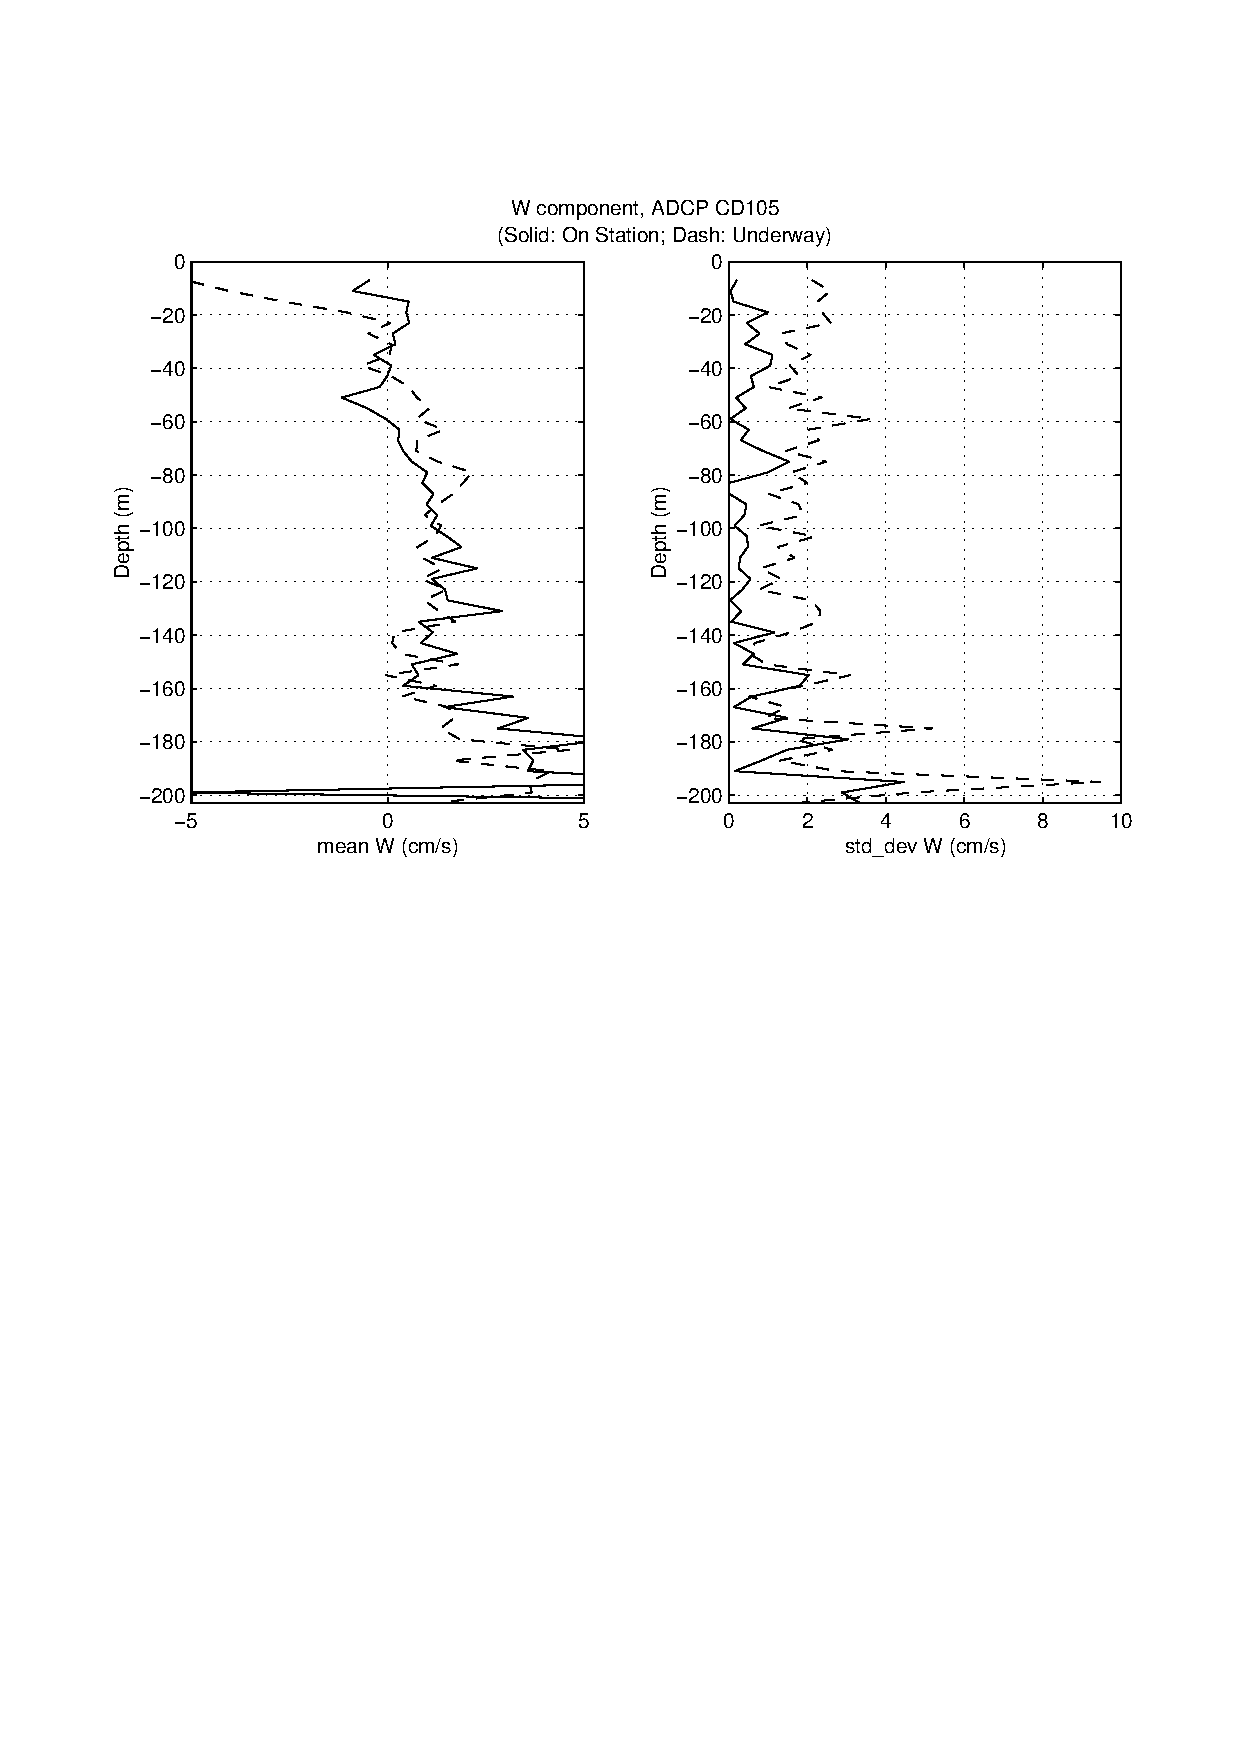
\includegraphics[width=7cm]{quality_W}%
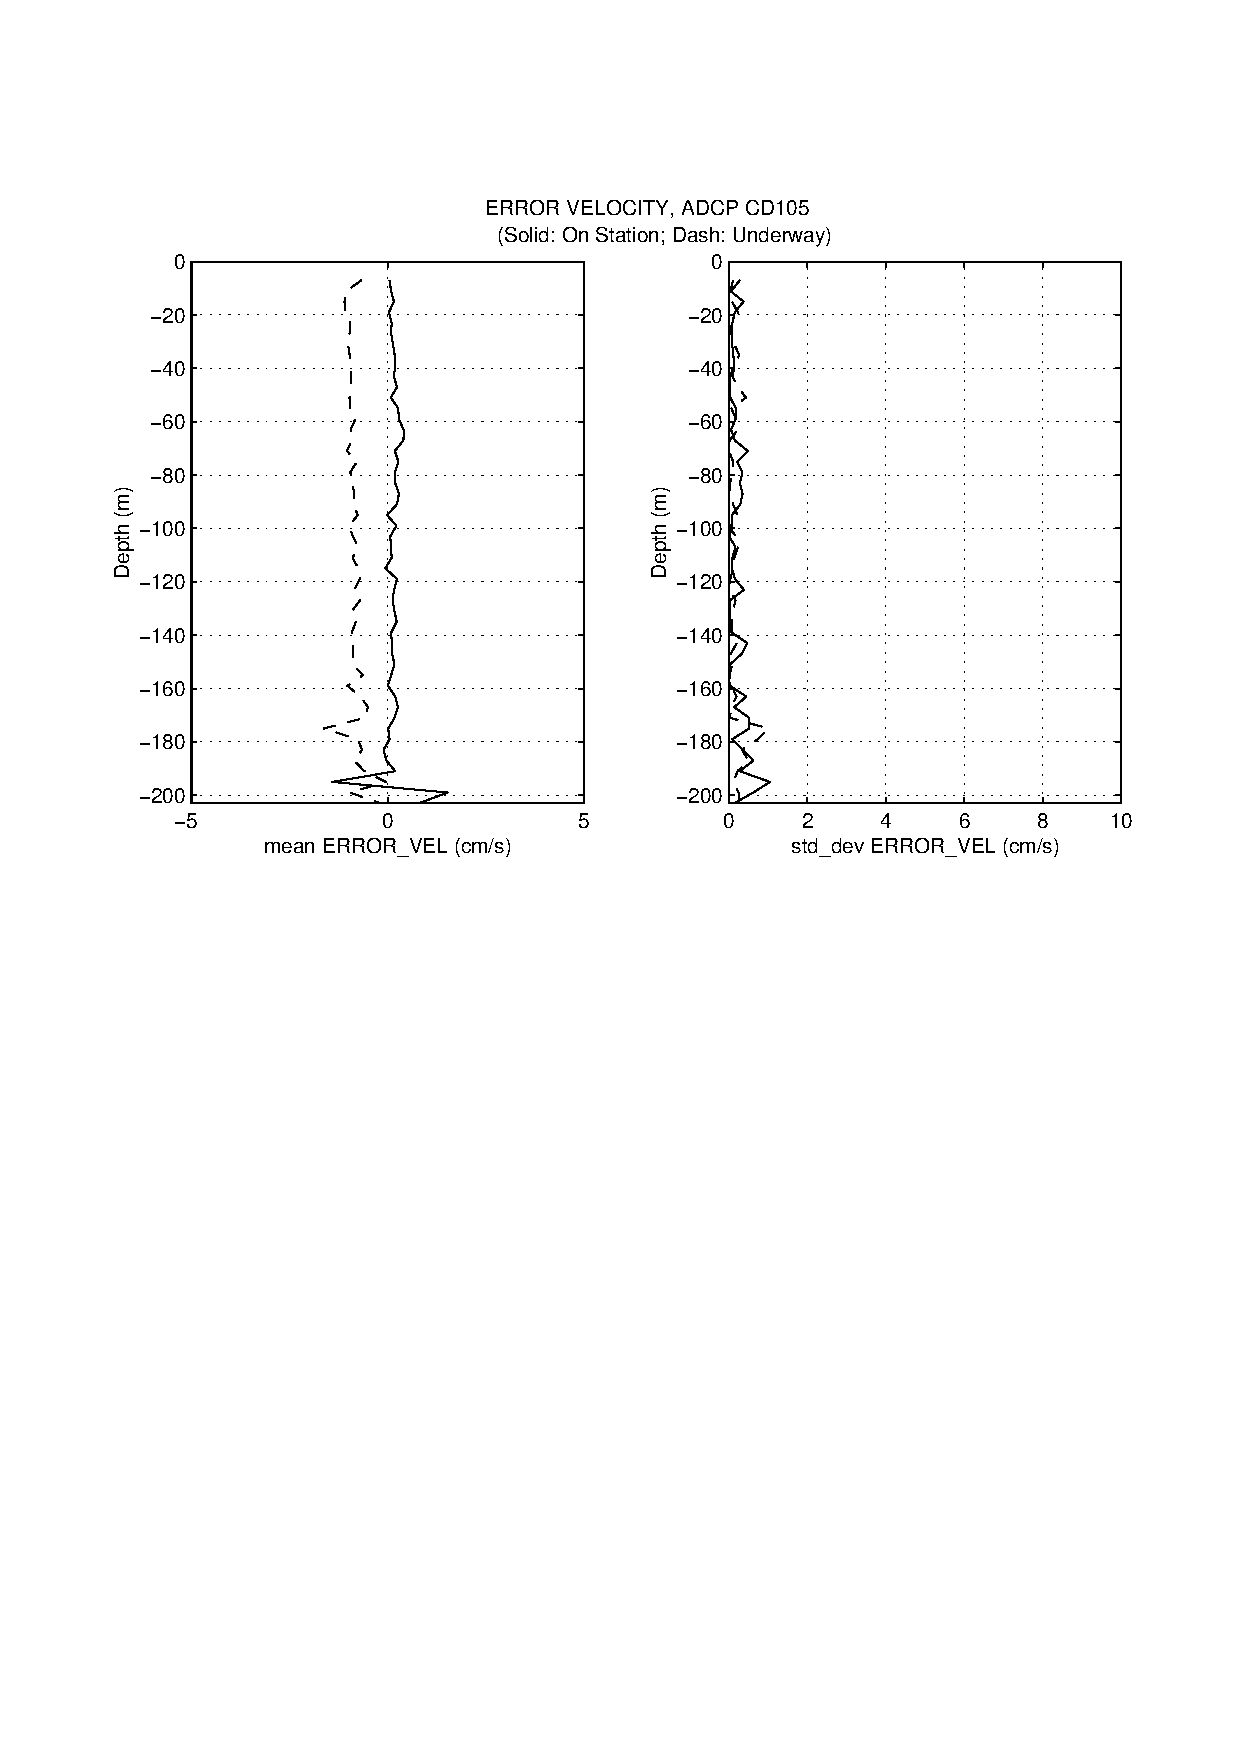
\includegraphics[width=7cm]{quality_E}
\caption{Plots of average value and standard deviation between the
5 minutes ensembles for underway and on station profiles of AGC,
PG, first vertical difference of horizontal components U and V,
vertical component of velocity and error velocity against depth.
For each plot the solid line represents on station data and the
dashed line, the underway data.} \label{fig:cd105qual}
\end{figure}
\paragraph{Calibration}\label{sec:springcal} Velocities relative to the ship must be adjusted
for orientation of the transducer relative to the gyro compass and
for any inaccuracy in the relative geometry of the four beams.
With accurate navigation information available during large
changes in ship's velocity, amplitude and angle errors can be
computed from the ADCP velocities during post processing
\cite{pollard89}. The method used was water track, which compares
the acceleration relative to the water, measured with the ADCP, to
the acceleration over the ground, calculated from navigation. The
calibration consists in the calculation of the amplitude ($\beta$)
and phase ($\alpha$) correction factor to the water track
velocities to be used subsequently in the Gyro correction,

\begin{equation}\label{eq:watertrack}
  U_c=\beta e^{i(\alpha \pi/180)}U_u,
\end{equation}
where suffix c and u stand for corrected and uncorrected velocity
in their complex form $U_c=u_c+iv_c$. The angle is specified
counterclockwise from the gyro compass forward axis (which should
be aligned with the ship's keel) to the transducer forward axis.
In the case of CD105 cruise, the values obtained for amplitude and
angle with their respective standard deviations for all
calibrations attempted are shown in Table~\ref{tb:cd105cal}. The
raw values were edited following a simple median criterion to
exclude outliers among $\beta$ and $\alpha$ estimates. Their time
evolution and frequency distribution are shown in
Fig~\ref{fig:cd105cal}. At worst (at highest ship speed of $\sim$
5\vel), the $\beta$ and $\alpha$ uncertainties imply an unknown
bias of 5\velc\, in velocity measurements.
\begin{table}[h]
  \centering
\begin{tabular}{llll}
\hline \hline
\multicolumn{2}{c}{$\beta \, \pm \, \sigma$} &
\multicolumn{2}{c}{$\alpha \, \pm \, \sigma$} \\ \cline{1-4}
1.02 & $\pm 0.01$ & -7.2 & $\pm 0.5 $\\
\hline \hline
\end{tabular}
  \caption{Calibration parameters for CD105}\label{tb:cd105cal}
\end{table}
\begin{figure}[t]
\begin{center}
\subfigure[]{
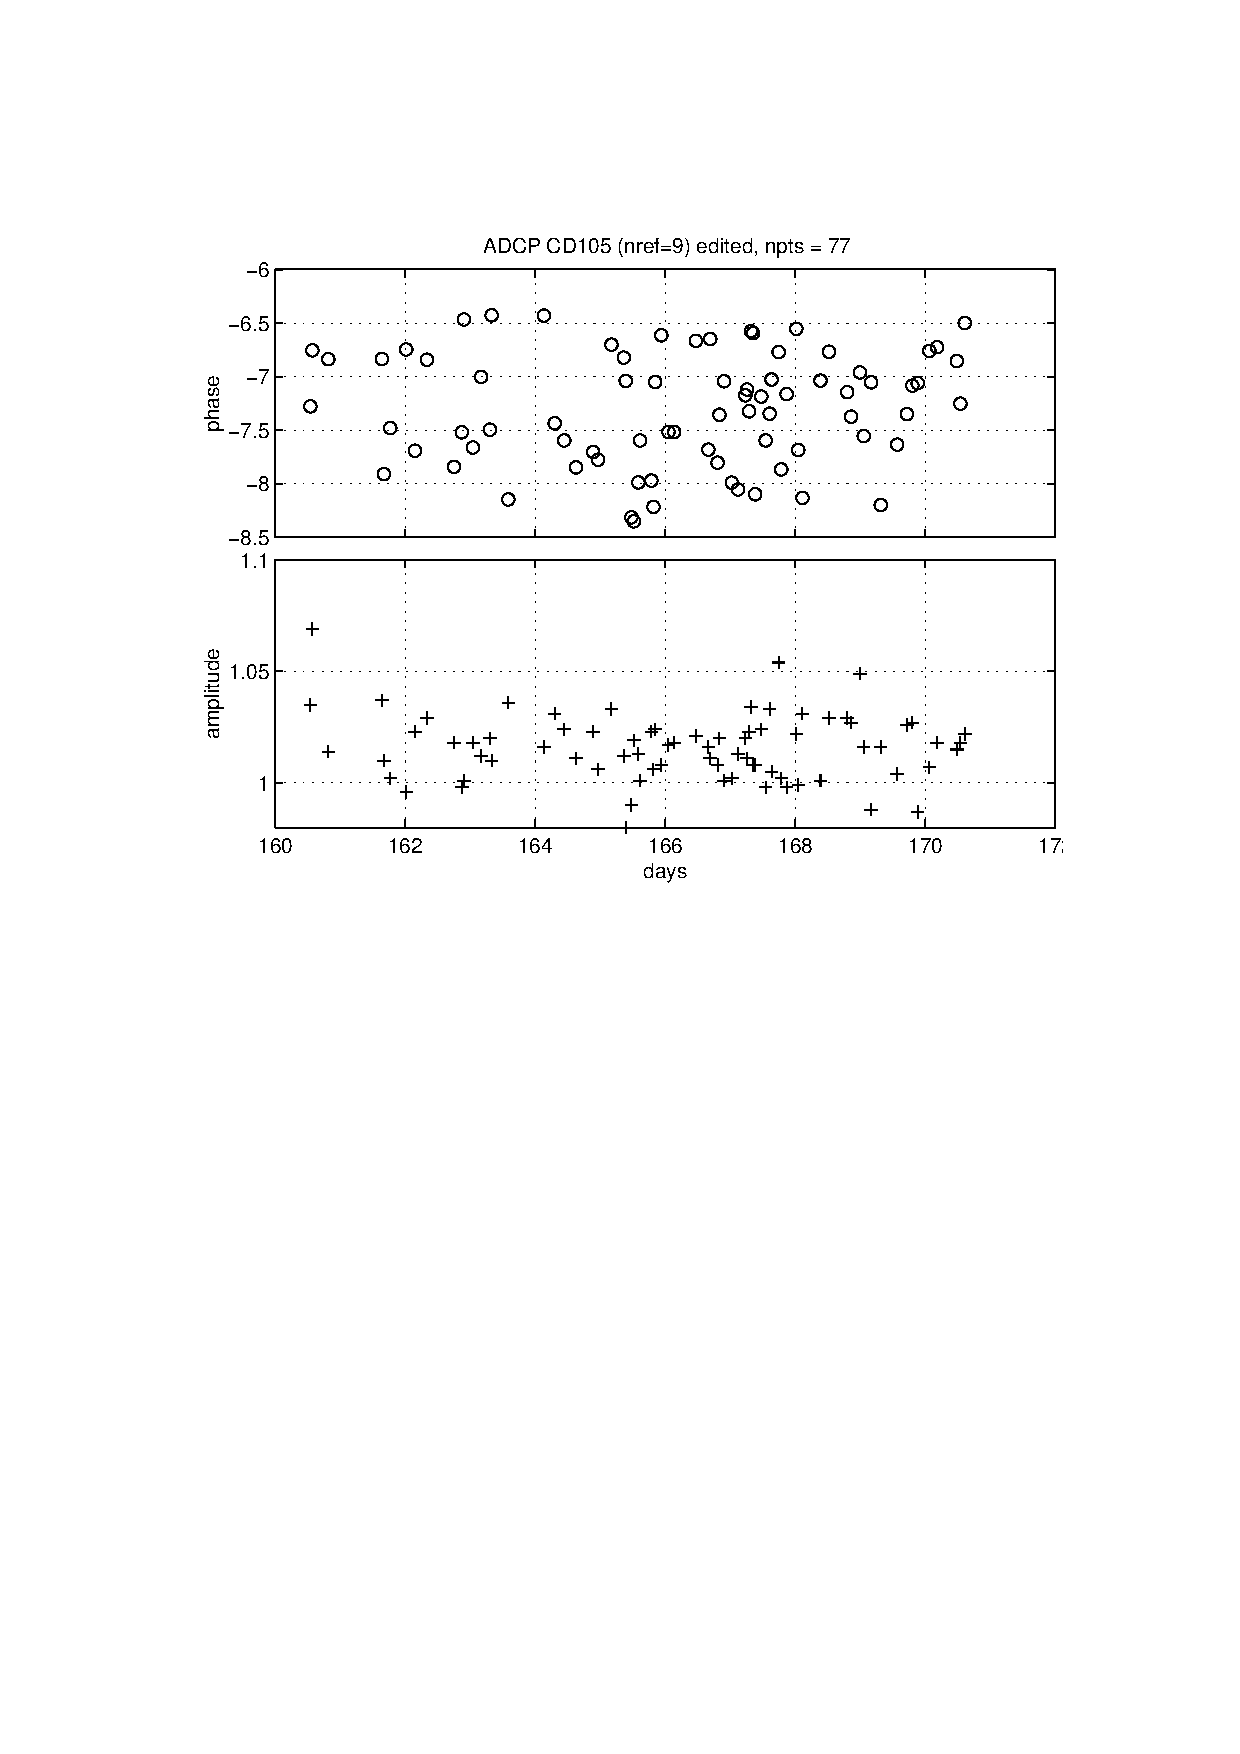
\includegraphics[width=7.cm,trim=0 0 0 0,clip]{cd105cal1}}
\subfigure[]{
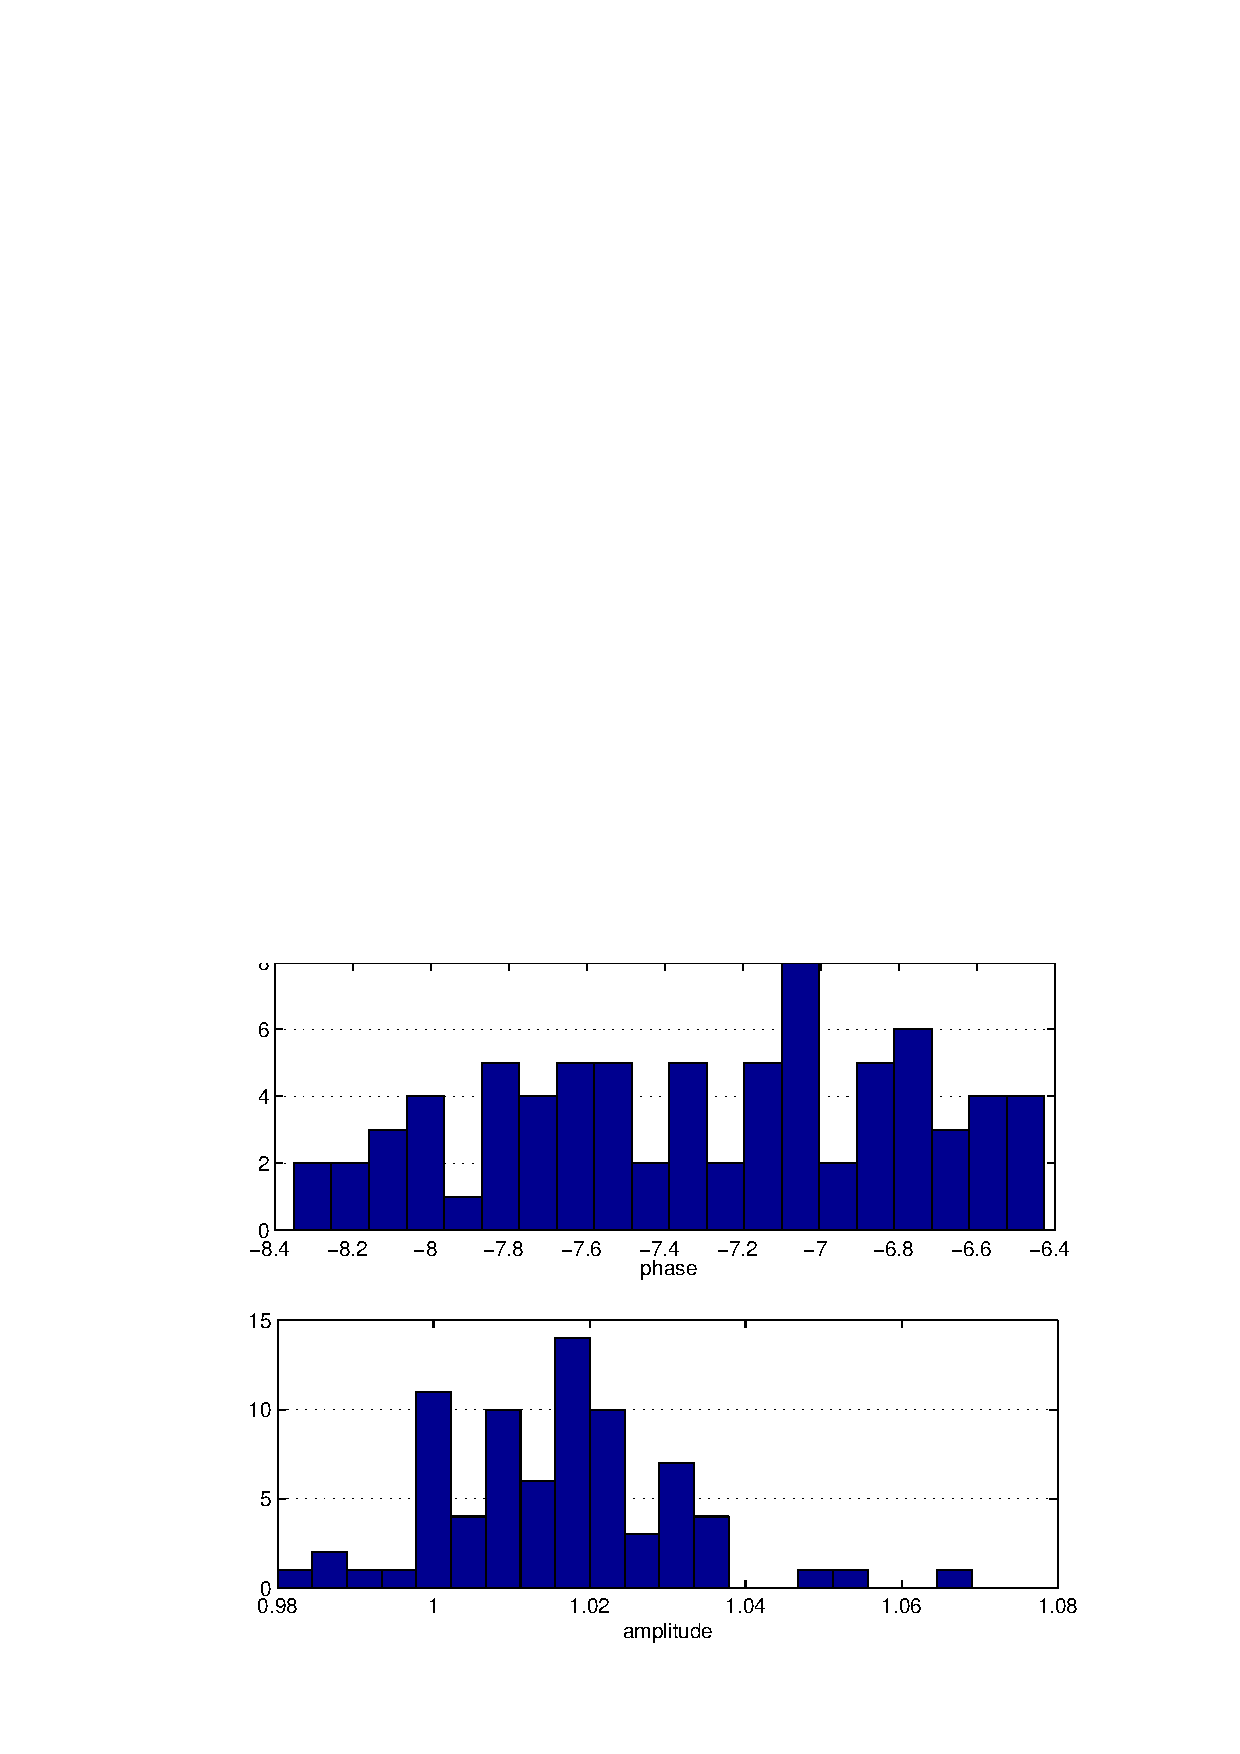
\includegraphics[width=7.cm,trim=0 -30 0 50,clip]{cd105cal2}}
\caption{Calibration parameters for CD105 cruise ADCP data.}
\label{fig:cd105cal}
\end{center}
\end{figure}


\paragraph{Navigation} The final step in processing ADCP data is the
introduction of navigation data, which are used to calculate the
ship's velocity and absolute water velocities. The absolute
reference layer velocity is the sum of the ship's speed over the
ground obtained from the navigation data, and the average relative
water velocity in the reference layer, measured by the ADCP.  This
layer is calculated with reference bins between 5 to 30. The data
used in this interval have a percentage good over 30. Once the
reference layer is obtained the data are interpolated and smoothed
with a Blackman window and a filter width of 30min as recommended
in \cite{codas}. Profile positions are also calculated from the
smoothed velocities. The final estimate of absolute velocities is
made by adding the shear profile for each ensemble to the
reference layer velocity. The step followed in this process were:
Obtain  the ship velocity relative to the reference layer.
Calculate the absolute ship velocity. Smooth and interpolate the
data to the ADCP ensemble times. Update the database. An example
of smoothed reference layer velocity can be seen in
Fig~\ref{fig:cd105ref}
\begin{figure}
  \centering
  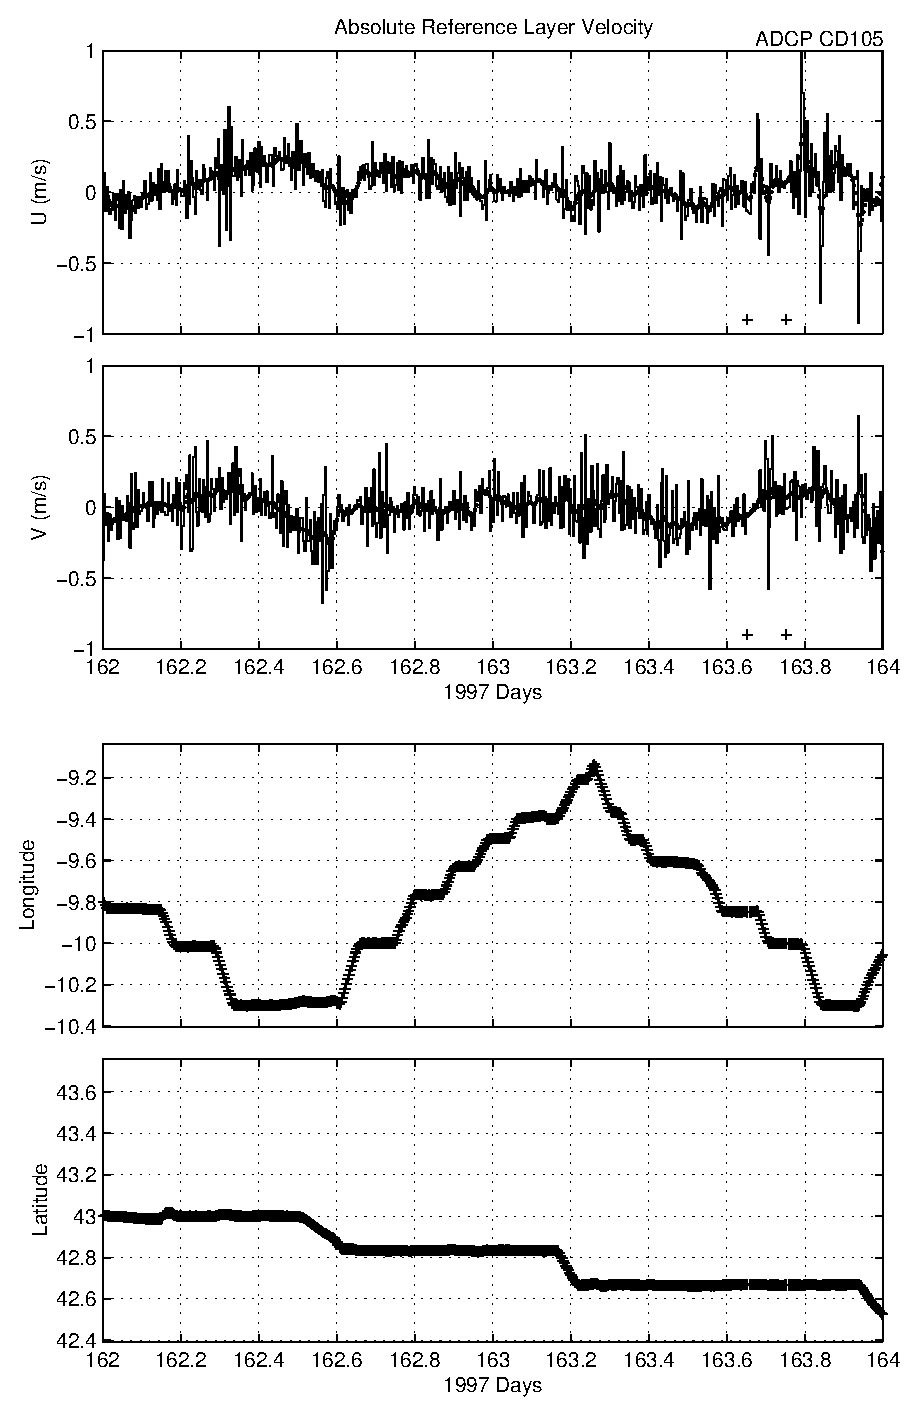
\includegraphics[width=13cm]{cd105ref}
  \caption{Smoothed reference layer velocity calculated over bins 5-30, and
  Latitude and Longitude time series from days 162-164.
  The data had been filtered to remove motions with time scales of less
  than 30min and rotated with the calibration parameters.
  Crosses at the bottom of the velocity panels
  indicate gaps in the GPS record}\label{fig:cd105ref}
\end{figure}

\subsubsection{Streamfunction Estimates of non-divergent flow}
In order to minimize the described limitations of the ADCP data
set due to instrumental errors, and the aliasing effects of tidal
and inertial signals, the streamfunction for the ADCP velocities
is derived (Eq.~\ref{eq:streamfunction}).
\begin{equation}\label{eq:streamfunction}
  \nabla^{2}\psi=\frac{\partial v}{\partial x} - \frac{\partial
  u}{\partial y}.
\end{equation}

The processing was similar to that reported in \citet{barth00} and
\citet{Pierce00}. Gridded fields of U and V components at selected
depths were built using a four-pass Barnes objective analysis (OA)
scheme \citep{barnes94,koch83}.  The gridded field is estimated by
iteratively applying a Gaussian-weighted average converging
towards the observed points. To account for the larger
uncertainties in the UW ADCP data, ship velocity weights were used
together with the distance-based weighting.  Although related to
the statistical optimal interpolation, this method does not
required prior specification of a covariance model for the
observed field.  The Barnes radii corresponded to 7km and 11km in
the X and Y directions so that scales larger than these were not
smoothed. The streamfunction was then calculated for the gridded
levels using the version III method of \citet{hawkins65}, also
described by \citet{carter87}, which represents an alternative way
of estimating the streamfunction values at the boundaries. The
method derives from the Helmholtz theorem (Eq.~\ref{eq:Helmholtz})
which allows the separation of a velocity field into a
non-divergent part and an irrotational component. $\overline{V}$
is the horizontal velocity, $K$ is the unit vertical vector,
$\psi$ is the horizontal streamfunction (the non-divergent part)
and $\eta$ is the horizontal velocity potential (the irrotational
part).
\begin{equation}\label{eq:Helmholtz}
  \overline{V}=K\times\nabla\psi+\nabla\eta.
\end{equation}
Taking the scalar product of Eq.~\ref{eq:Helmholtz} with n, the
unit outward normal vector, we get,
\begin{equation}\label{eq:streamboundary}
  \frac{\partial\psi}{\partial
  s}=-\overline{V}_{n}+\frac{\partial\eta}{\partial n},
\end{equation}
where $s$ is the distance along the boundary in a counterclockwise
direction, and $\overline{V}_{n}$ is the velocity normal to the
boundary. By integrating it we solve for the $\psi$ values at the
boundary that will be used in the streamfunction calculations,
rather than using the observed velocity field, which need not be
non-divergent given the measurement noise. However, the boundary
values of $\eta$ need to be calculated first by solving
Eq.~\ref{eq:etaboundary}, for the velocity potential forced by the
observed field of divergence.
\begin{equation}\label{eq:etaboundary}
  \nabla^{2}\eta=\nabla\cdot\overline{V}.
\end{equation}
Boundary conditions of $\eta=0$ were imposed. In this way, the
total kinetic energy of the $\psi$ field is maximized while
minimizing the amount of energy in the $\eta$ field
\citep{carter87}.

The Poisson solver developed by \citet{cummins94} was used to
solve Poisson equations
Eq.~\ref{eq:streamfunction}-\ref{eq:etaboundary}. The solver uses
the capacitance matrix method and handles Dirichlet boundary
conditions in an irregular domain. Non-divergent vectors are
derived from the gridded streamfunction and then interpolated back
to their original locations using improved Akima bivariate
interpolation \citep{akima96} The Barnes OA and the streamfunction
derivation together amount to a method of systematically applying
conservation of mass throughout a region \citep{Pierce00}. The
derivatives were calculated with central differences in the
interior points while forward difference was used at the
boundaries. Trapezoidal numerical integration was used in all
integral calculations.

\begin{figure}[!ht]
\centering \subfigure[]
{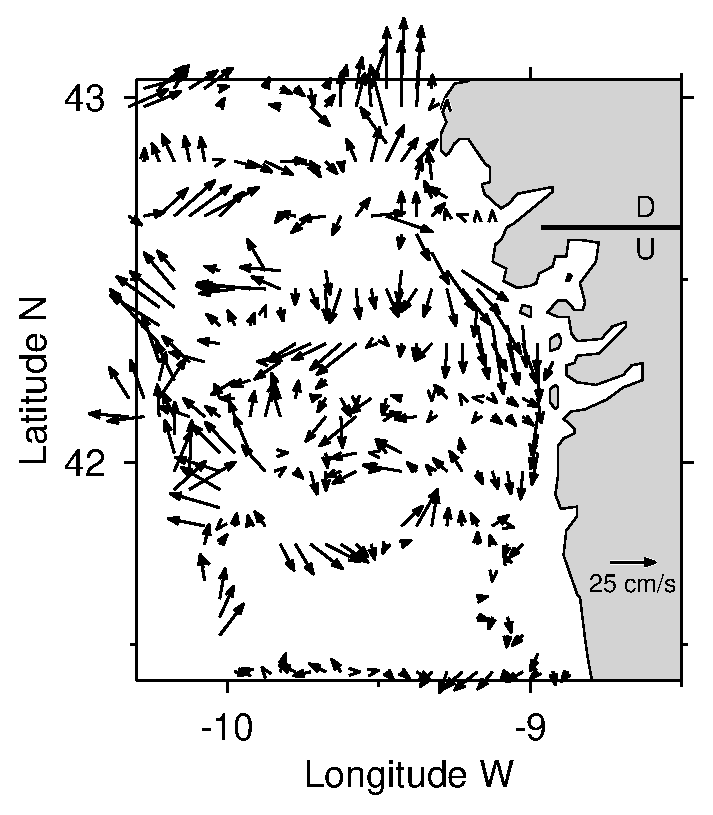
\includegraphics[width=6cm]{cd105adcpraw_51}} \subfigure[]
{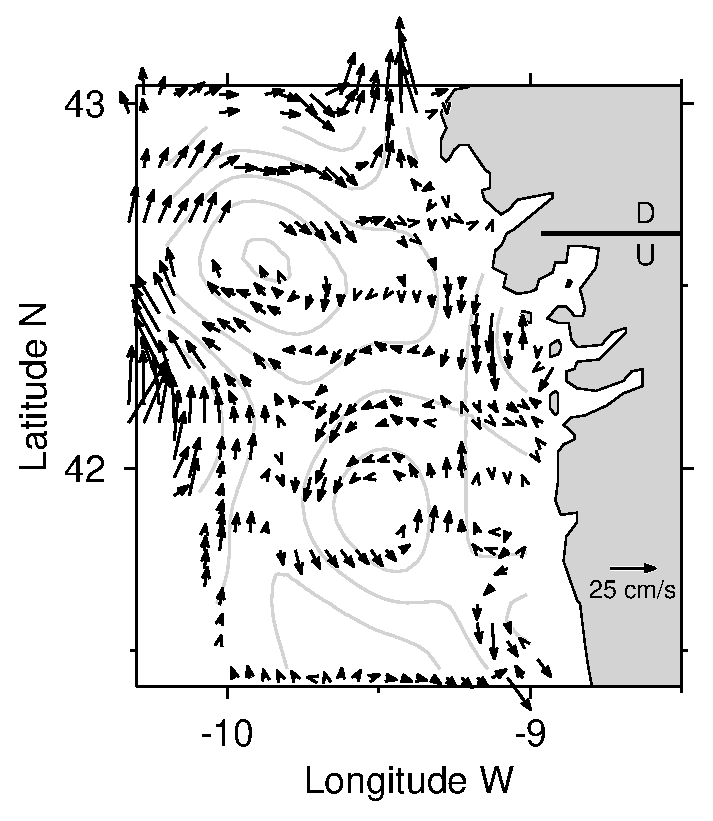
\includegraphics[width=6cm]{cd105stream_51}} \caption{Example of
(a) vectorised ADCP data with minimum averaging of 10min and 12m
in the vertical centred at 51m and (b) non-divergent ADCP current
vectors superimposed on transport streamfunction contours with a
$0.01\times 10^{6}$\tra contour interval. The line on land
indicates the area sampled under upwelling (U) and downwelling (D)
conditions.} \label{fig:cd105_stream}\end{figure}

An example of the vectorised ADCP data and non-divergent current
vectors centred at 51m is shown in Fig.~\ref{fig:cd105_stream}.
ADCP current vectors (Fig~\ref{fig:cd105_stream}a) were averaged
in cells of 0.05x0.05\deg. The non-divergent field clearly
reproduces the large scale features seen in the raw field. The
offshore poleward flow, coastal southward jet and the two eddies
are all well defined in the non-divergent field. It is important
to bear in mind that strong wind changes took place during the
cruise, mostly affecting the nearshore region, and the
non-divergent field is a smoothed version of the raw field.

\section{Results}
\subsection{SST and wind conditions prior, during and after the cruise}
The CD105 cruise took place during the Galician transition from
the poleward flow dominated winter regime to the upwelling summer
regime. The weekly SST composite images in Fig~\ref{fig:cd105sst}
correspond to 1-7 June, coincident with leg A, and 29-05 July,
nine days after the completion of the cruise. Their resolution is
about 4km and they are the median, pixel by pixel, of all early
morning satellite passes over the week. Spurious structures and
patchiness can have been introduced by the merging process due to
clouds and transient structures and so the figures have to be
considered cautiously. In Fig~\ref{fig:cd105sst}a the coastal warm
waters extend to the 200m isobath, with temperature decreasing
northwards, while a second warm tongue of similar temperature lies
offshore of the 1000m isobath.  The two tongues appear to converge
south of 41\deg N. Eddy like structures with scales of 30km are
evident in the offshore tongue (E1-E3 ) but were no longer visible
in subsequent images possibly due to the storm on 6-8 June (e.g.
Fig~\ref{fig:cd105winds}). In the next two weeks, the offshore
branch of the warm tongue weakened and receded, and on the third
week it did not extend beyond 42.5\deg N Fig~\ref{fig:cd105sst}b.
The coastal tongue disappeared and was replaced by a coastal band
of upwelled water extending to 200m Fig~\ref{fig:cd105sst}b.

\subfiguretopcaptrue \subcapnoonelinetrue
\begin{figure}[t]
\centering \subfigure[]
{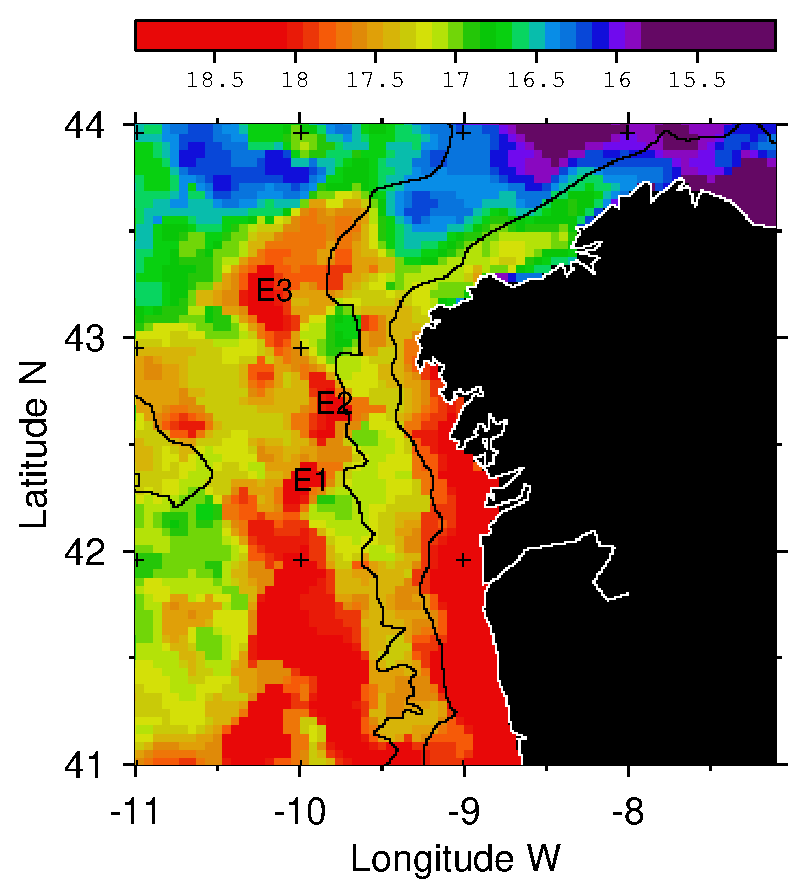
\includegraphics[width=6cm]{ga970601-0607medfincol}}%
\subfigure[] {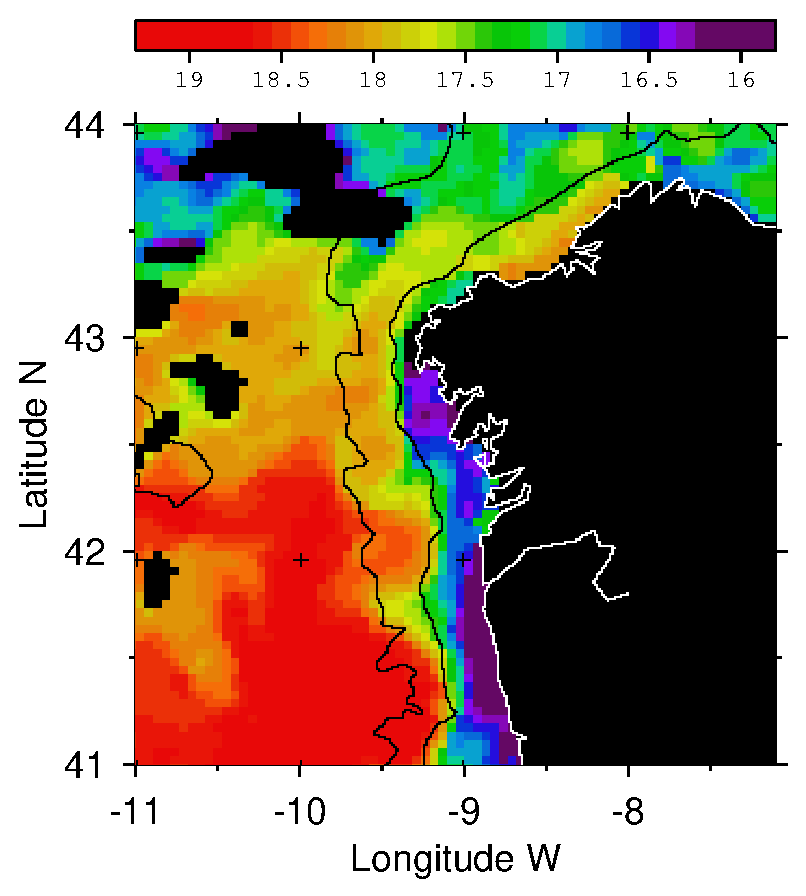
\includegraphics[width=6cm]{ga970629-0705medfincol}}
\caption{SST weekly averaged images from a)1-7 and b)29-05 July
1997 corresponding to leg A and 9 days after the end of cruise
CD105. Eddies have been numbered with an E prefix. The 200 and
1000m isobath are included. Note the different temperature scale.}
\label{fig:cd105sst}\end{figure}

Coastal winds (Fig~\ref{fig:cd105winds}) were recorded at three
locations along the Galician coast at Vilanova, Finisterre and
Corrubedo (Fig~\ref{fig:cd105stations}) for the months of June and
July. The period of the cruise is indicated in the figure. The
wind flows predominantly along the direction of the coast and
spatial differences are expected due to the complex coastline of
the region. Although these might not be representative of the more
complex large scale winds (e.g. Chapter~\ref{ch:winds}) they can
give an indication of predominantly upwelling or downwelling
favourable winds. During leg A until 13 June conditions were
downwelling favourable with peak winds of 15\vel\, and 12\vel\, at
Vilanova and Corrubedo, respectively, on 6-8 June when a storm hit
the region. Thereafter conditions were upwelling favourable with
variable weak winds of 6\vel\, until 13 July, and remained
strongly upwelling favourable in excess of 10\vel\, afterwards.
Hence, 4 days after the start of leg B, the regime changed from a
strongly downwelling scenario to a weak upwelling one, which had
an impact in the nearshore stations and affected the synopticity
of sampling. This will be discussed later in the chapter.
\begin{figure}[hct]
\centering
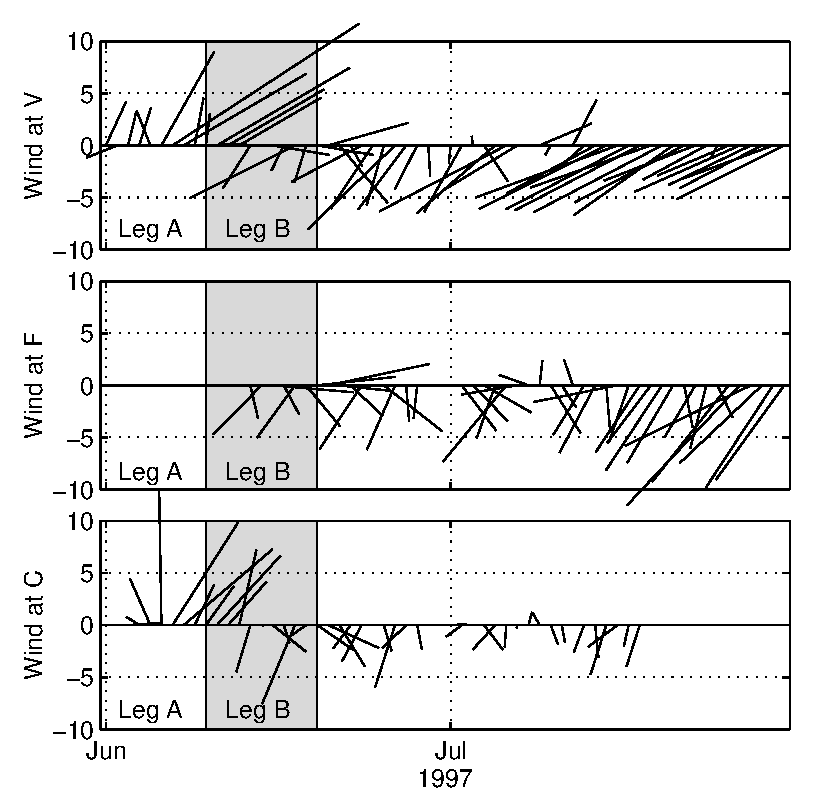
\includegraphics[width=8cm]{winds97cd105}
\caption{Daily coastal winds from Corrubedo (C), Finisterre (F)
and Vilanova (V). The time of the two Cruise legs is indicated in
the graph. The sticks point in the direction of the wind with the
North in the positive Y axis.} \label{fig:cd105winds}
\end{figure}

Six hourly estimates of upwelling index at 42\deg N, 9\deg W from
May to August (Fig.~\ref{fig:cd105upindx}) were derived from the
Fleet Numerical Meteorology and Oceanography Center synoptic wind
fields obtained from the NOAA Pacific Fisheries Environmental
Laboratory [{\it http://www.pfeg.noaa.gov}]. The upwelling indices
were calculated using Bakun's method \citep{Bakun73}.
Figure~\ref{fig:cd105upindx} clearly shows the shift in the wind
regime in agreement with the local winds. Except for brief
episodes of upwelling favourable winds at the beginning of May,
weak or downwelling favourable winds were common throughout the
second half of May and early June. On 14 June, winds became
upwelling favourable and remained so until the end of the record.
\begin{figure}[hct]
\centering
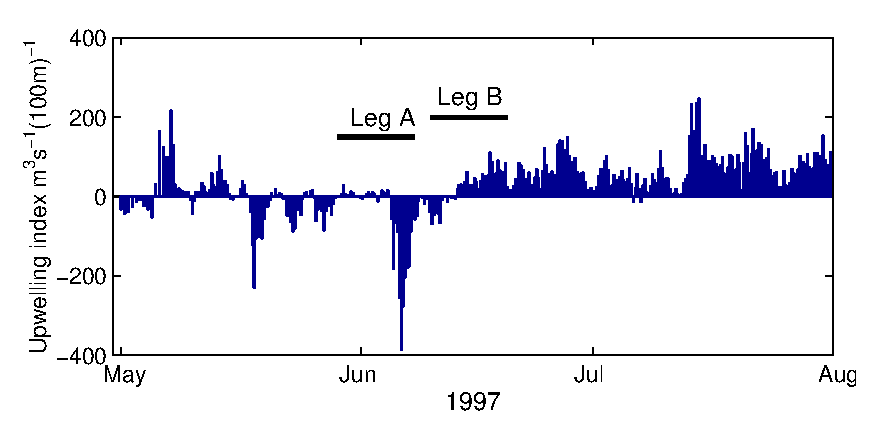
\includegraphics[width=8cm]{upindex97}
\caption{Six hourly estimates of upwelling index at 42\deg N,
9\deg W, \tra(100m)$^{-1}$. Data from NOAA Pacific Fisheries
Environmental Laboratory. } \label{fig:cd105upindx}
\end{figure}

\FloatBarrier
\subsection{Horizontal Fields}
\subsubsection{Near-Surface (5m) fields}
The near-surface salinity distribution (5m) recorded from the
thermosaligraph for legs A and B are shown in
Fig~\ref{fig:cd105ths}. Although it is difficult to consider them
as true synoptic fields in the light of the wind changes occurring
during the cruise they will be discussed as snapshots. The
temperature fields are not discussed here as they showed a strong
diurnal heating that masked any of the spatial structures. The
salinity in this region can be used as a circulation tracer
because the T/S characteristics in the upper layer (top 100m) are
roughly perpendicular to the isopycnals (Fig~\ref{fig:cd105ts}a).

During leg A (Fig~\ref{fig:cd105ths}a) the salinity range was
small in most of the area (36.08-35.70psu) with the exception of
an isolated low salinity region marked as ``L'' in the graph where
it reached values of 35.4psu. Salinity generally decreased with
latitude, and meridional differences were larger than zonal ones.
The SST composite image of leg A has a signature similar to the
near surface salinity field, with warmer temperatures related to
higher salinities. The region of highest salinity ($>36psu$) in
the SW corner of the graph corresponds to an area of high
temperatures in Fig~\ref{fig:cd105sst}a and the warm tongue
extending from it has a rough equivalent in the salinity field,
both turning inshore at $\sim$42.4\deg N. Near the location of E2
(Fig~\ref{fig:cd105sst}a) in Fig~\ref{fig:cd105ths}a, a local
salinity maximum exists. The low salinity region ``L'' is part of
a relatively low salinity tongue which seems to have its origin in
the Rias Bajas (Fig~\ref{fig:largebathy}), between 42.2\deg and
42.5\deg N, although more southern origins can not be ruled out.
The tongue turns southwards at -9.5\deg W, rather than northwards
as would have been expected from freshwater plume dynamics. Note
that along that longitude a colder water band can be seen in
Fig~\ref{fig:cd105sst}a parallel to the offshore warm tongue.

In leg B, the sampling included coastal stations at depths $<100m$
and the salinity range widened to include lower values (36-30.5
psu). The period was characterized by weak upwelling favourable
winds except for the time of the three northernmost sections. The
shoreward limit of leg A decreased in salinity in leg B
(Fig~\ref{fig:cd105ths}b), which showed even lower values
nearshore, particularly south of 42.75\deg N. This led to the
formation of a strong salinity front which was enhanced south of
42.25\deg N due to the presence of the high salinity tongue
offshore (P in the graph) with $\triangle S>0.4psu$. The high
salinity tongue P broadened during leg B and split at 42.25\deg N,
one branch turning offshore at that latitude, while the other
progressed northwards only to turn offshore further north. The
high salinity structure E is now better defined with values
$>38.85$psu. The low salinity tongue (L in leg A), had shifted
slightly northward, decreased in salinity and extended offshore to
-10\deg W south of E.
\begin{figure}[h]
\centering \subfigure[]
{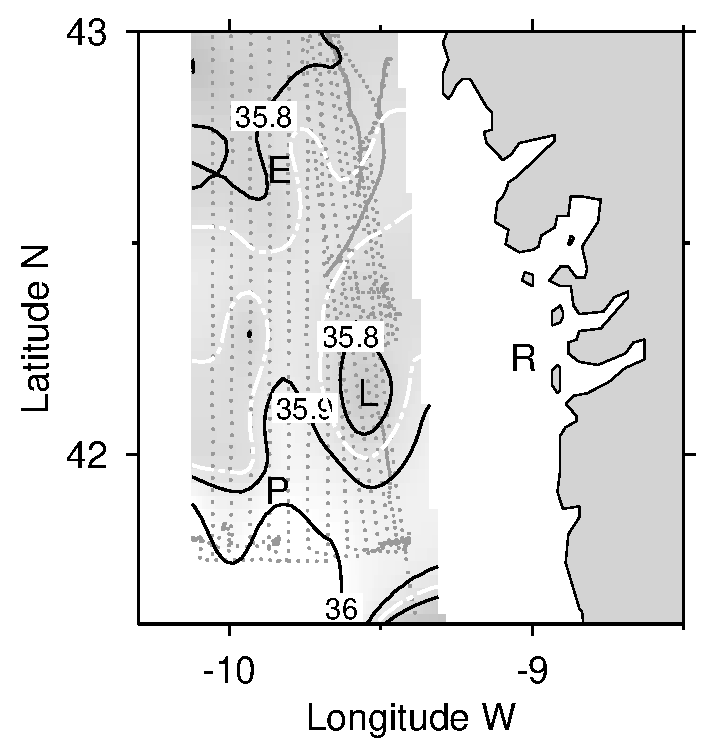
\includegraphics[width=6cm]{cd105a0sal}}%
\subfigure[] {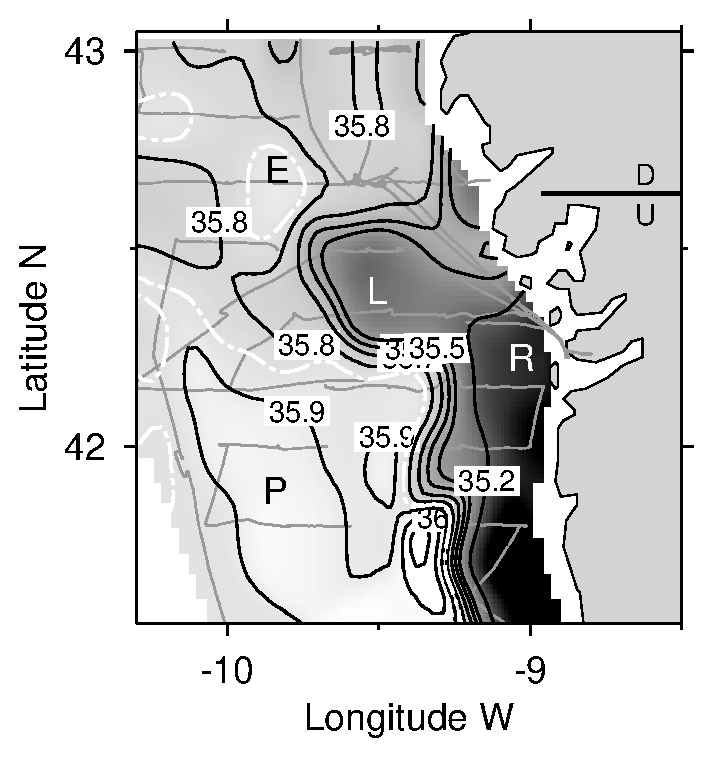
\includegraphics[width=6cm]{cd105b0sal}}
\caption{Salinity distribution at 5m as recorded by the
thermosalinograph from a)leg A and b)leg B. The isosaline of 35.85
appears as a white dashed line. The structures identified in leg B
are indicated as E (eddy), P(poleward flow) and R (fresh water
runoff) and are included in a) for reference. A low salinity
region found in leg A is marked as L. Darker shading indicates
lower salinity. The line on land indicates the area sampled under
upwelling (U) and downwelling (D) conditions. }
\label{fig:cd105ths}\end{figure}
\begin{figure}[ht]
\centering \subfigure[]{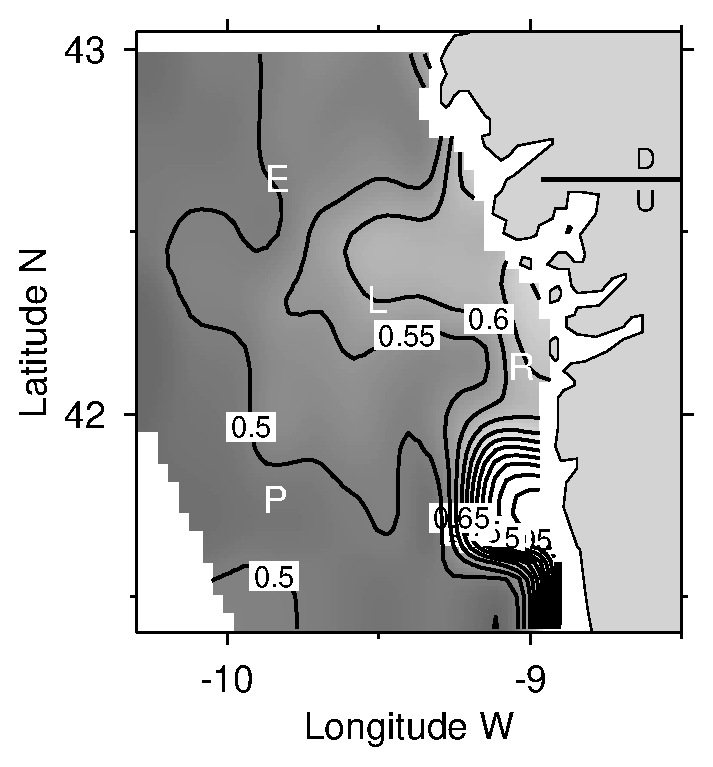
\includegraphics[width=6cm]{cd1055chl}}
\subfigure[]{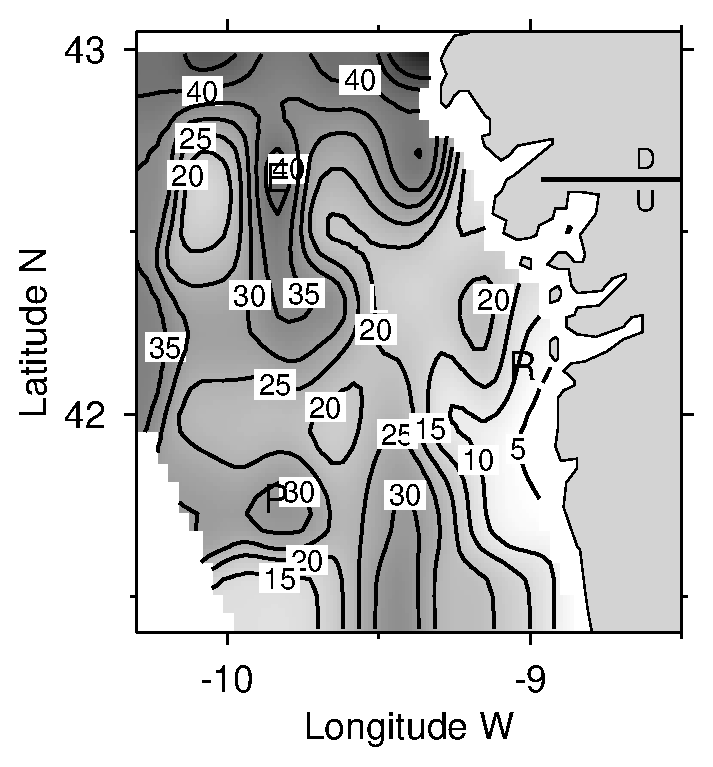
\includegraphics[width=6cm]{mixedlayer01}}
\caption{a) Fluorescence distribution (in Volts) at 5m as measured
by the CTD from leg B. Darker shading correspond to lower
fluorescence values. b) Distribution of surface mixed layer depth
using criteria of $\Delta \sigma_{t}=0.1$\dens. The line on land
indicates the area sampled under upwelling (U) and downwelling (D)
conditions.}\label{fig:cd105chl5m}
\end{figure}

The near surface (5m) un-calibrated fluorescence data from leg B
(Fig~\ref{fig:cd105chl5m}a) resembles the salinity field with high
fluorescence values related to low salinity. The salty tongue P
had associated low fluorescence values ($<0.5$V), as had the
northern offshore waters. Values were higher close to the mouth of
the Rias and the Mi\~{n}o River, where the highest values were
measured ($>1$V), but  decreased rapidly offshore on scales of
$<20$km. The previously identified low salinity tongue L can be
seen in Fig~\ref{fig:cd105chl5m} as a region of fluorescence in
the range 0.55-65V extending offshore near 42.4\deg N.

The mixed layer distribution (Fig~\ref{fig:cd105chl5m}b) was
calculated using the density difference with the surface, with the
criteria $\Delta \sigma_{t}=0.1$\dens, which represents a measure
of the layer that has been recently mixed \citep{brainerd95}.
Maximum depths ($>40m$) were measured in the northern limit in
association with the poleward flow while minimum values were
encountered nearshore south of 42.25\deg N. The latter corresponds
to the region influenced by the freshwater runoff from the
Mi\~{n}o river. The low salinity plume L had typical mixed layer
depths of 20m. The centre of the eddy E was characterized by
deeper mixed layer depths than surrounding waters by as much as
20m.

\begin{figure}[ht]
\begin{widefig}{-.5cm}{-.7cm}
\centering \subfigure[]
{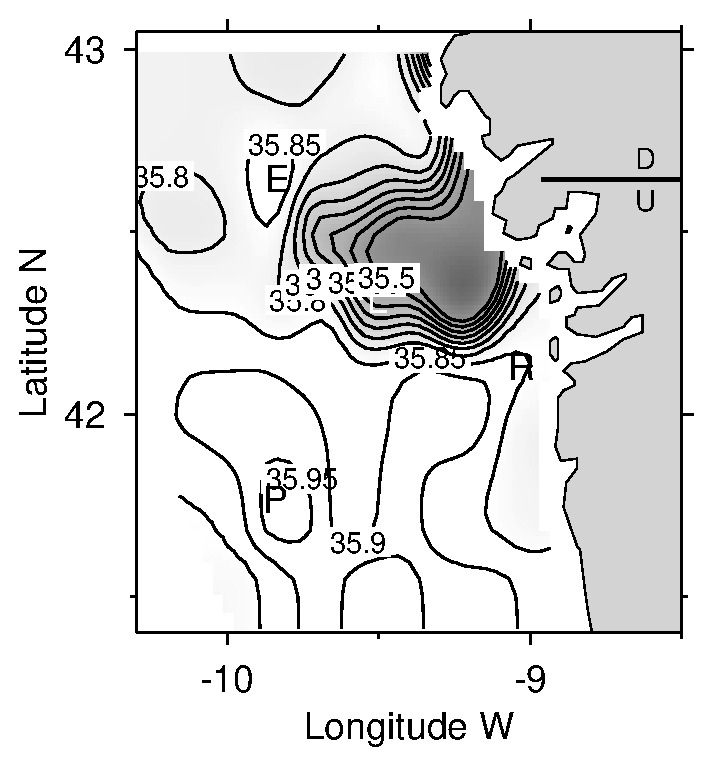
\includegraphics[trim=0 0 0 -15,clip,width=5.3cm]{cd105sal_15}}%
\subfigure[] {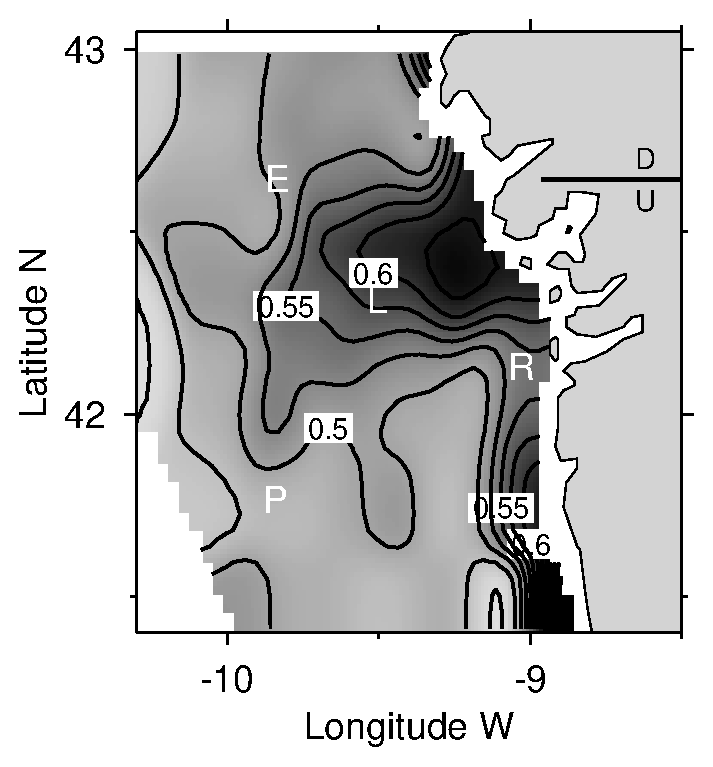
\includegraphics[trim=0 0 0
-15,clip,width=5.3cm]{cd105chl_15}} \subfigure[]
{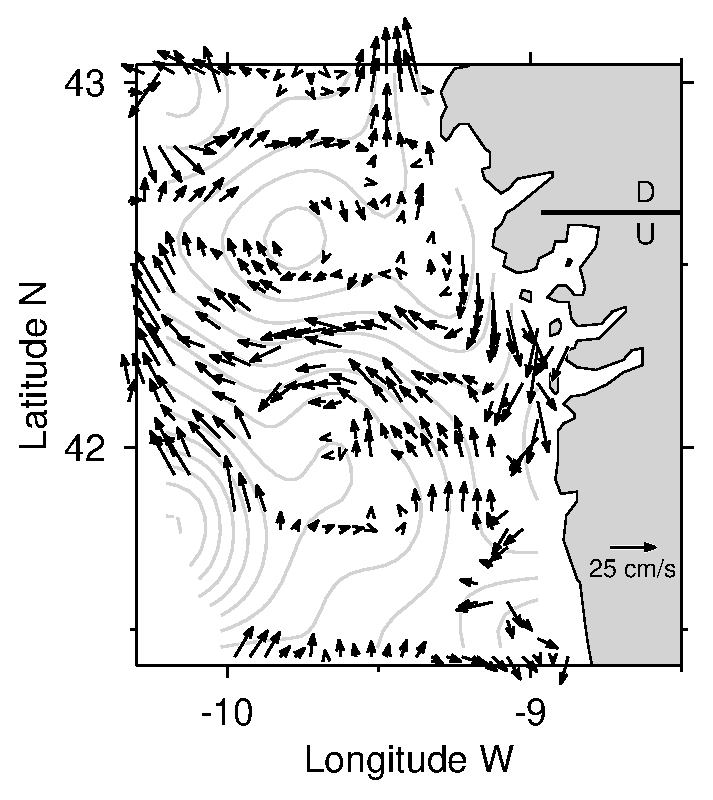
\includegraphics[width=5.3cm]{cd105stream_15}}
\caption{Near-surface (15m) properties during Leg B 10-20 June
1997. (a) Salinity; darker shading corresponds to lower salinity.
(b) Fluorescence in Volts; darker shading correspond to higher
values. (c) Non-divergent ADCP current vectors with minimum
averaging of 10min and 12m in the vertical centred at 15m
superimposed on transport streamfunction contours with a
$0.01\times 10^{6}$\tra contour interval. The line on land
indicates the area sampled under upwelling (U) and downwelling (D)
conditions.} \label{fig:cd105_15m}
\end{widefig}\end{figure}

\subsubsection{Near-Surface (15m) fields} Horizontal fields at the
level of the shallowest reliable ADCP bin (12m bin centred at 15m
depth) are shown in Fig~\ref{fig:cd105_15m}. The salinity and
fluorescence contours (\ref{fig:cd105_15m}a-b) show some
fundamental differences when compared to the 5m fields. The
freshwater coastal band south of 42.15\deg~N has now disappeared
although a narrow band of high fluorescence is still visible 15km
off the coast. The salty tongue P at this depth shows two
branches, the offshore branch, which was clearly present at 5m in
Fig~\ref{fig:cd105ths}a and b, and a coastal branch, only slightly
evident at 5m, running along the slope as far as 42.15\deg~N. The
low salinity region L still extends offshore but at a more
northern position and with minimum values ($<35.5$) now closer to
shore than at the surface. The eddy E is visible and relatively
high salinity is found nearshore north of 42.7\deg N and offshore
as at the suface. The fluorescence field shows a similar pattern
to the 5m level, however higher values extend further offshore.
Part of the high fluorescence plume turns southwards at 9.75\deg W
42\deg N, while a smaller tongue turns northward offshore the high
salinity eddy E. The poleward branching is also noticeable in the
fluorescence data south of 42\deg N.

The non-divergent current field and overlaid contours of
streamfunction transport are shown in Fig~\ref{fig:cd105_15m}d.
The main structure is the broad contorted poleward flow with
maximum velocities of $>$25\velc. Much of its transport appears to
enter the region west of 10\deg W where no measurements were
available at this level. Observations at deeper levels
(Fig.~\ref{fig:cd105_stream}a) show this inflow clearly. The
inflow fed the offshore poleward flow (0.04Sv) and only 0.02Sv
came from the south to form the coastal branch with velocities up
to 15\velc. The two branches correspond to the salinity and
fluorescence distribution of Figs.~\ref{fig:cd105_15m}a-b. The
coastal poleward current meets the southward coastal current with
velocities up to 25\velc\ at 42.3\deg N (0.03Sv) and veers
offshore to merge with the offshore branch. This change in
direction from northward to southward coastal current could also
be related with the shift in wind forcing and could represent a
temporal change. Most of the poleward flow (0.08Sv) leaves the
region westward between 42\deg-42.5\deg N but 0.03Sv proceeds
northwards with lower salinity after having mixed with the low
salinity coastal current. Anticyclonic circulation was associated
with the high salinity eddy E involving 0.01Sv. The flow further
splits into the offshore and the coastal poleward current (0.02Sv)
reaching velocities up to 25\velc. At this shallow level the
current field was affected by the wind reversal and so the coastal
poleward flow observed in the first three northern lines might
have later reversed with the wind to form part of the coastal
southward jet observed in the south. A more detailed discussion on
the nearshore variability during the cruise is presented later in
the chapter.

\subsubsection{Sub-surface fields}

The salinity field below the mixed layer ( at 50m,
Fig~\ref{fig:cd105_51m}a) shows the offshore salty tongue along
the western limit of the grid more clearly. Salinity was higher
(36$psu$) in the offshore branch than in the separate coastal
branch (35.95-35.90$psu$). The high salinity eddy E appears
shifted to the west. No sign of the coastal freshwater plume seen
at shallower levels is apparent at 50m. Lower salinity
($<35.9psu$) is found mainly north of 42.5\deg N at the coast, and
further north offshore.

The fluorescence field (Fig~\ref{fig:cd105_51m}b) also lacks the
high coastal values seen in
Fig~\ref{fig:cd105chl5m}a-\ref{fig:cd105_15m}b. It exhibits a
patchy distribution of high fluorescence centres (0.5-0.65V) which
seem related to the offshore poleward flow and the eddy E. These
centres were not present at shallower levels.

\begin{figure}[ht]
\begin{widefig}{-.5cm}{-.7cm}
\centering \subfigure[]
{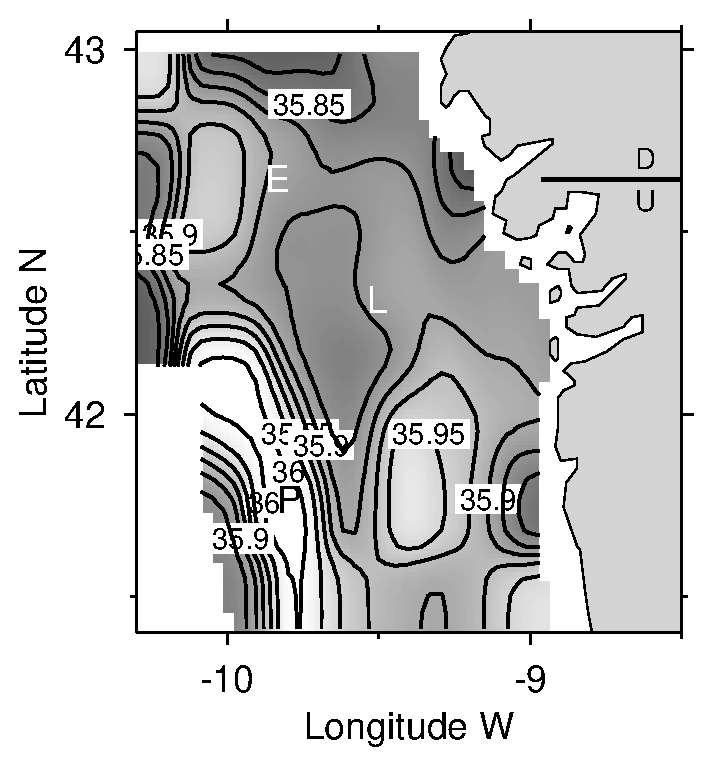
\includegraphics[trim=0 0 0 -15,clip,width=5.3cm]{cd105sal_51}}%
\subfigure[] {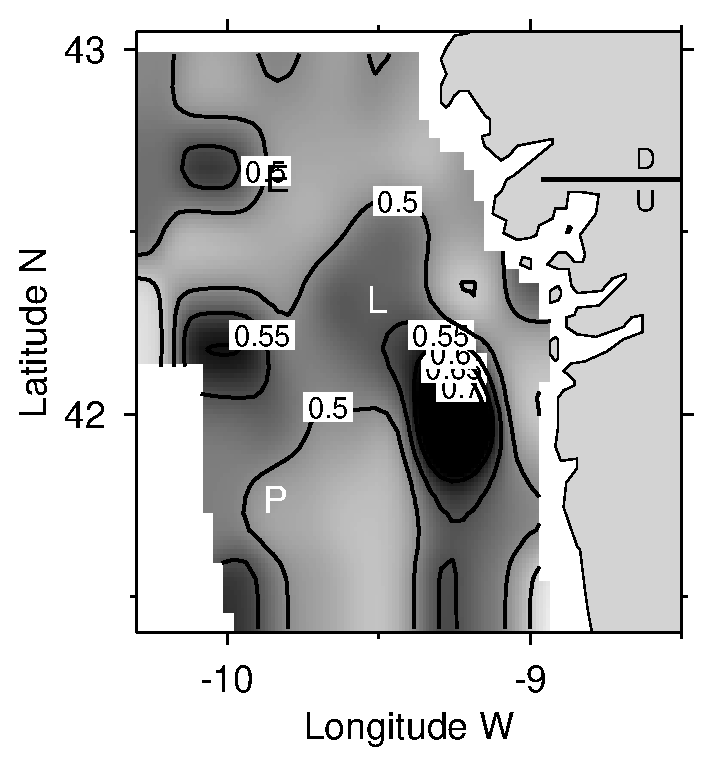
\includegraphics[trim=0 0 0
-15,clip,width=5.3cm]{cd105chl_51}} \subfigure[]
{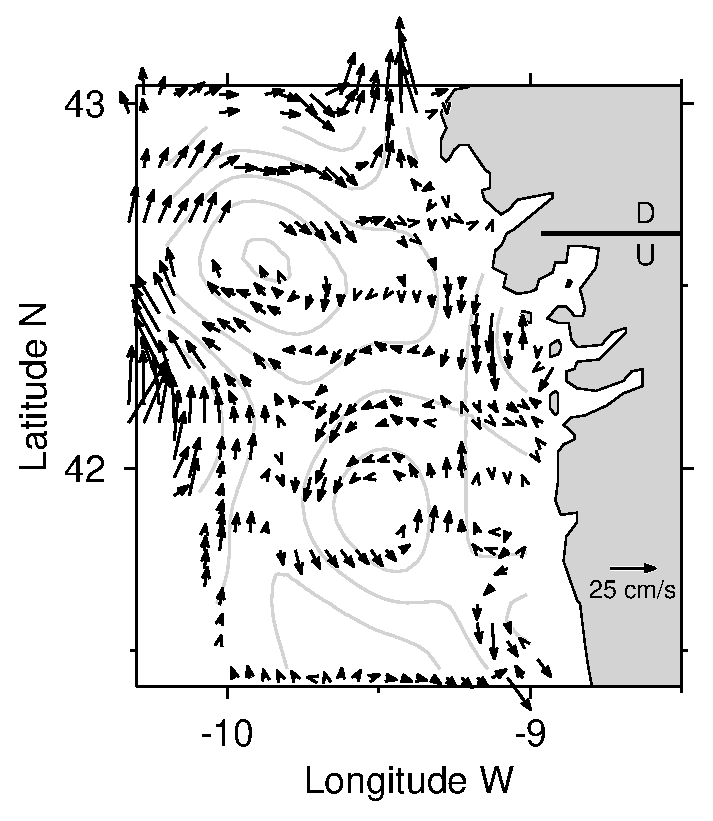
\includegraphics[width=5.3cm]{cd105stream_51}}
\caption{Sub-surface (50m) properties during Leg B 10-20 June
1997. (a) Salinity; darker shading corresponds to lower salinity.
(b) Fluorescence in Volts; darker shading correspond to higher
values. (c) Non-divergent ADCP current vectors superimposed on
transport streamfunction contours with a $0.01\times 10^{6}$\tra
contour interval. The line on land indicates the area sampled
under upwelling (U) and downwelling (D) conditions.}
\label{fig:cd105_51m}%
\end{widefig}\end{figure}

The non-divergent field (Fig~\ref{fig:cd105_51m}d) shows weaker
circulation at this level. Nonetheless the offshore poleward flow
is still strong ($\sim$20-25\velc\,) at the western limit of the
sampled region with a transport of at least 0.03Sv. The northern
coastal poleward branch has similar transport to 15m (0.02Sv) and
the same holds for the anticyclonic circulation of the eddy E
(0.01Sv). However, some of the offshore waters return to the shelf
north of the eddy, and join the weak coastal southward flow. The
more inshore poleward flow in the south appears more part of a
cyclonic re-circulation than a continuous current.

\begin{figure}[ht]
\centering \subfigure[]
{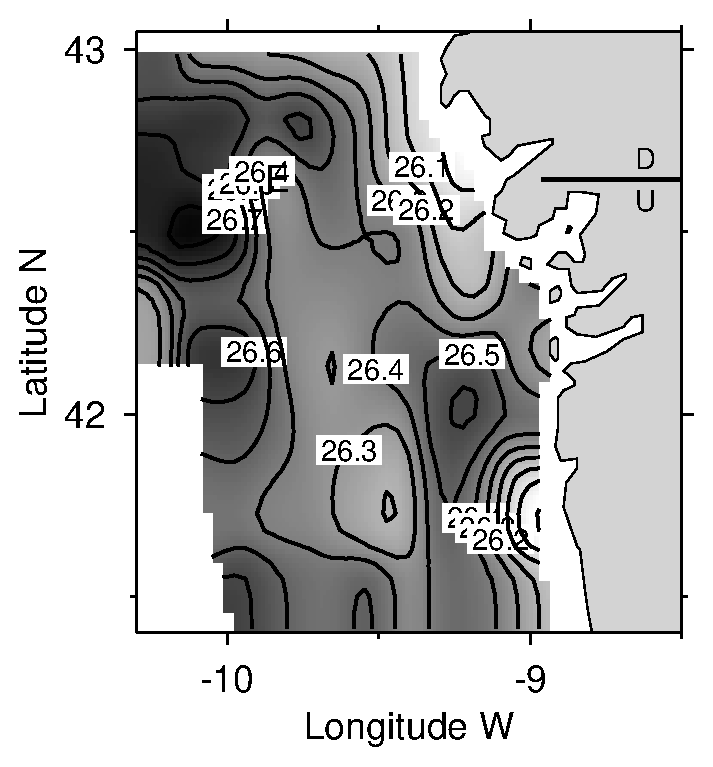
\includegraphics[width=6cm]{cd105den_51}}%
\subfigure[] {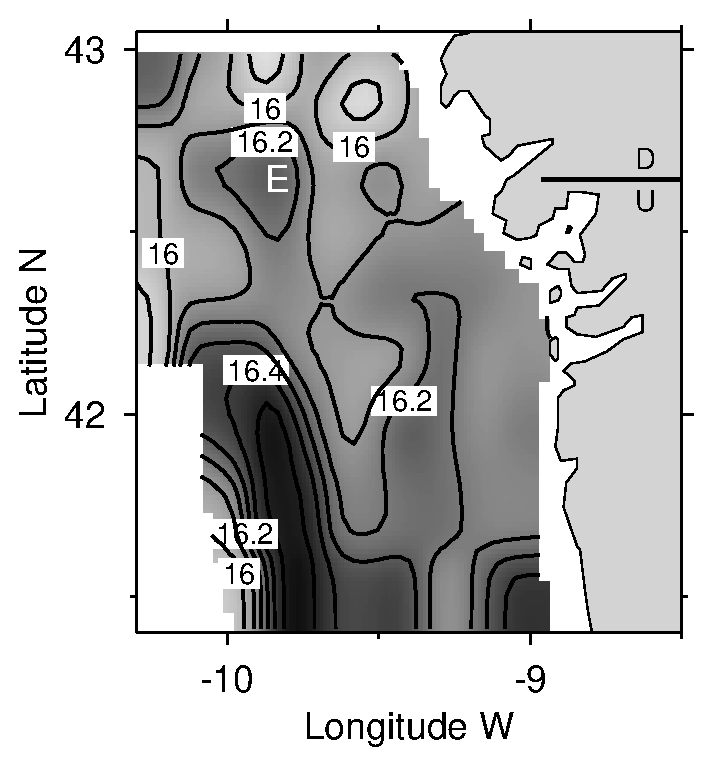
\includegraphics[width=6cm]{cd105tem_den26_4}}
\caption{Sub-surface (50m) contour of (a) Density and distribution
of (b) Temperature at $\sigma_{t}=26.4$\dens isopycnal. The line
on land indicates the area sampled under upwelling (U) and
downwelling (D) conditions.} \label{fig:cd105_26.4}
\end{figure}
The density distribution at 50m (Fig~\ref{fig:cd105_26.4}a) was
similar to the temperature distribution at this depth as
temperature is the controlling factor over salinity. The 50m level
is in or just below the thermocline at most of the off-shelf CTD
stations. Small deviations in the pycnocline caused by internal
tides and waves can significantly contaminate the temperature
distributions near this depth level. The temperature is therefore
plotted on the isopycnal surface (26.4\dens) which best represent
the base of the mixed layer. The resultant distribution
(Fig~\ref{fig:cd105_26.4}b) resembles the salinity distribution at
50m. Higher temperatures were associated with the high salinity
offshore poleward flow as expected and the centre of the eddy E is
now positioned east of the high salinity anomaly in better
agreement with the non-divergent current vectors.


Similar structures are present at deeper levels. The offshore
salty and warm poleward flow was present down to 200m
(Figs.~\ref{fig:cd105_100m}a-~\ref{fig:cd105_200m}a), its salinity
difference with surrounding waters decreasing with depth. The more
nearshore poleward flow was completely separated from the offshore
branch at 100m by a low salinity-low temperature band running
parallel to the coast (Fig.~\ref{fig:cd105_100m}a-b). Remnants of
the coastal branch (warm and salty pools) were found north and
south of the Rias Bajas at 100m but disappeared at deeper levels
(Fig~\ref{fig:cd105_150m}a,b-~\ref{fig:cd105_200m}a,b). The eddy E
was present down to 250m with highest associated anomalies 0.1psu
(0.8\deg) salinity (temperature) at 150m
(Fig~\ref{fig:cd105_150m}a-b) suggesting it is a deep seated
feature, though smaller than a typical SWODDY \citep{Pingree92b}.



\begin{figure}[th]
\begin{widefig}{-.5cm}{-.7cm}
\centering \subfigure[]
{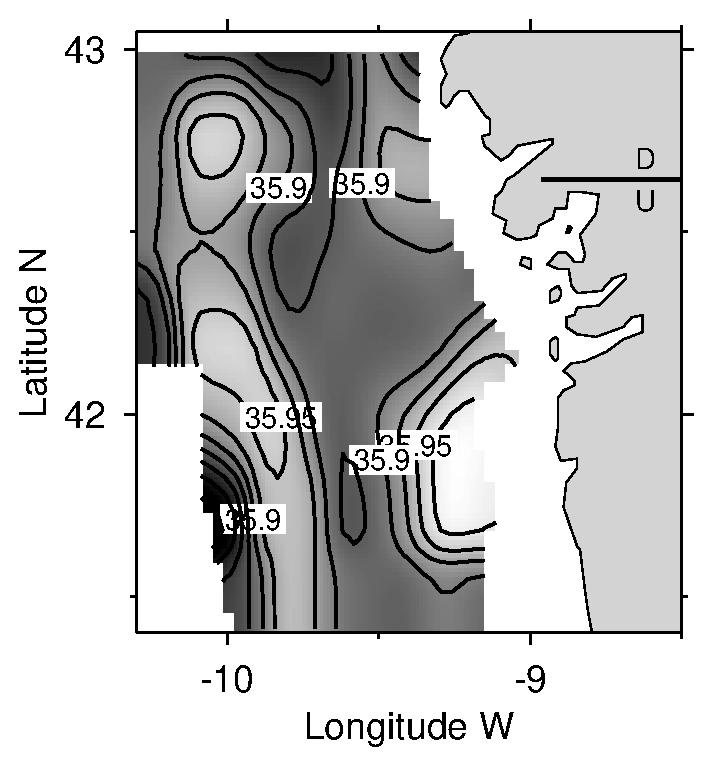
\includegraphics[trim=0 0 0 -15,clip,width=5.3cm]{cd105sal_100}}%
\subfigure[] {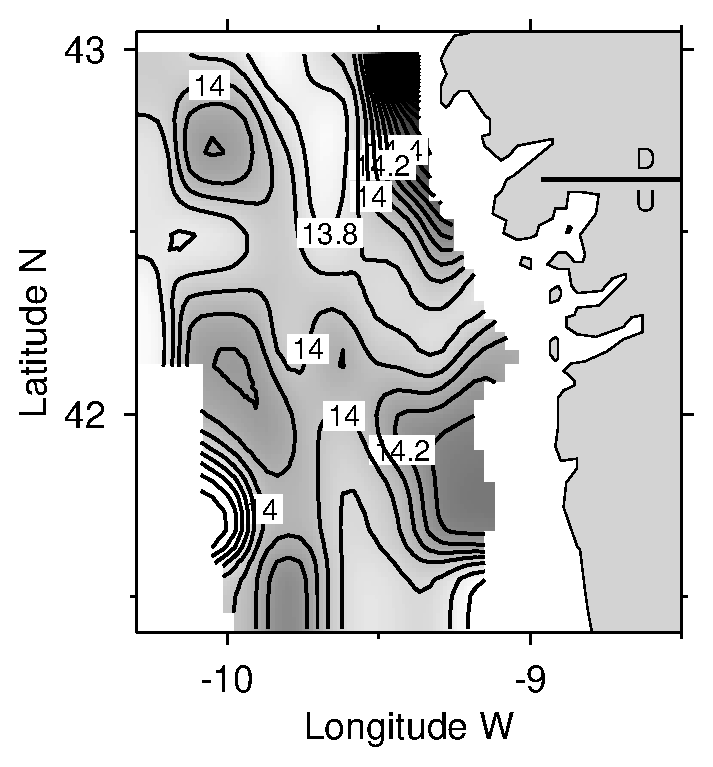
\includegraphics[trim=0 0 0
-15,clip,width=5.3cm]{cd105tem_100}} \subfigure[]
{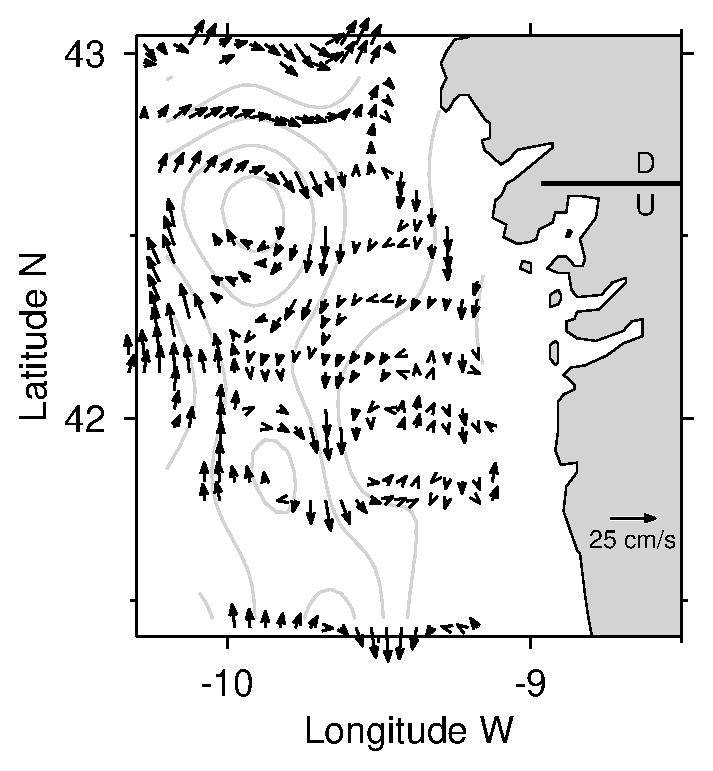
\includegraphics[width=5.3cm]{cd105stream_107}}
\caption{Sub-surface (100m) properties during Leg B 10-20 June
1997. (a) Salinity; darker shading corresponds to lower salinity.
(b) Temperature; darker shading correspond to warmer temperatures.
(c) Non-divergent ADCP current vectors superimposed on transport
streamfunction contours with a $0.01\times 10^{6}$\tra contour
interval. The line on land indicates the area sampled under
upwelling (U) and downwelling (D) conditions.}
\label{fig:cd105_100m}\end{widefig}\end{figure}

%poleward flow visible; remains of the coastal poleward flow
%visible. None opposite rias bajas, maybe due to wind funnelling at
%the rias. Presence of the continue southward flow off the slope.
%Generates possibly due to the offshore migration of the poleward
%flow instigated by the onset of upwelling winds and offshore
%advection of freshwaters. They provide stratification that would
%also delay the rising of isopycnals.
%
\begin{figure}[th]
\begin{widefig}{-.5cm}{-.7cm}
\centering \subfigure[]
{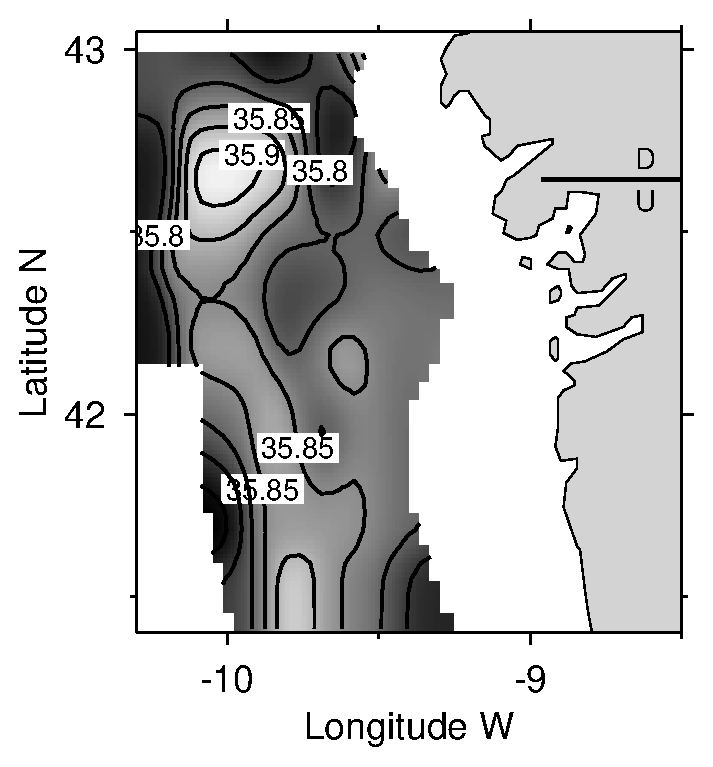
\includegraphics[trim=0 0 0 -15,clip,width=5.3cm]{cd105sal_150}}%
\subfigure[] {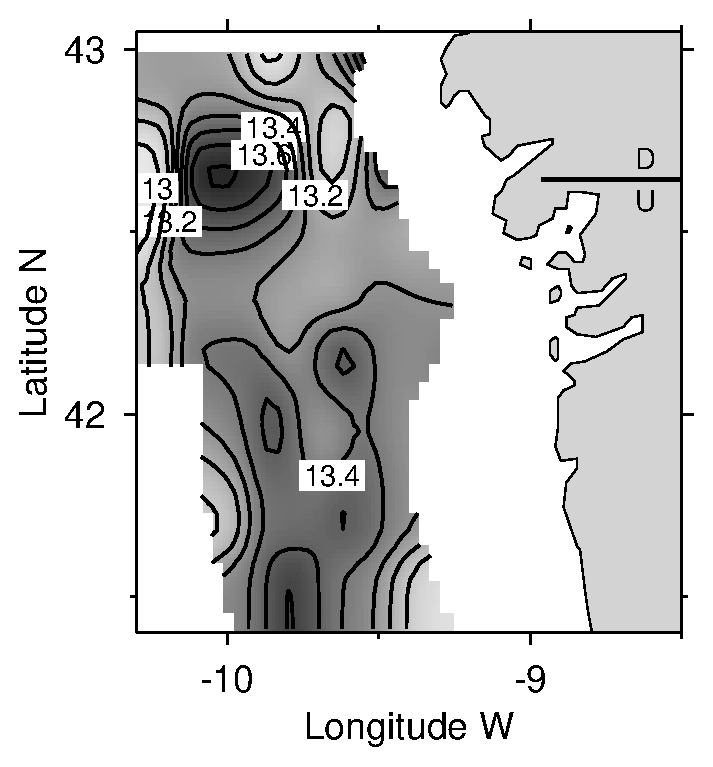
\includegraphics[trim=0 0 0
-15,clip,width=5.3cm]{cd105tem_150}} \subfigure[]
{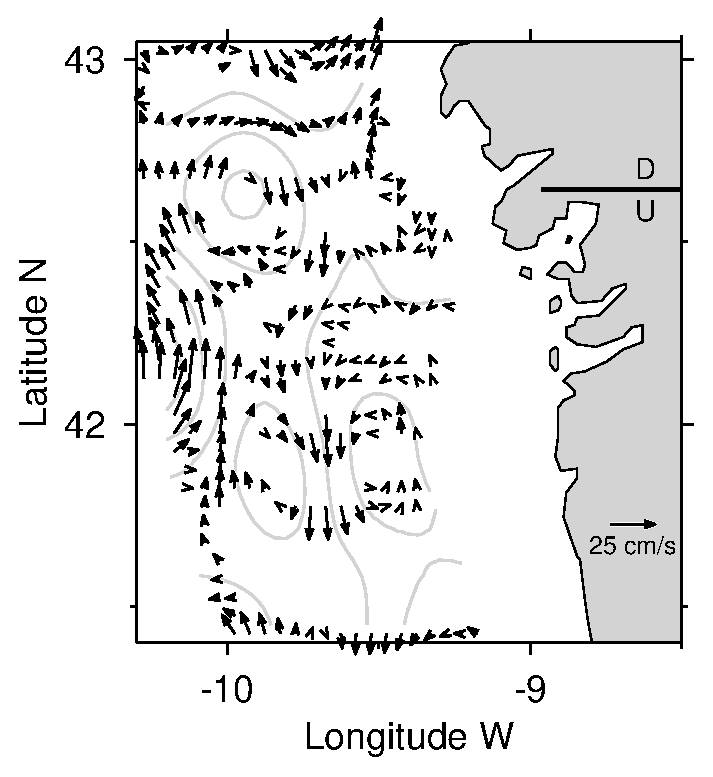
\includegraphics[width=5.3cm]{cd105stream_155}}
\caption{Sub-surface (150m) properties during Leg B 10-20 June
1997. (a) Salinity; darker shading corresponds to lower salinity.
(b) Temperature; darker shading correspond to warmer temperatures.
(c) Non-divergent ADCP current vectors superimposed on transport
streamfunction contours with a $0.01\times 10^{6}$\tra contour
interval. The line on land indicates the area sampled under
upwelling (U) and downwelling (D) conditions.}
\label{fig:cd105_150m}\end{widefig}\end{figure}

\begin{figure}[th]
\begin{widefig}{-.5cm}{-.7cm}
\centering \subfigure[]
{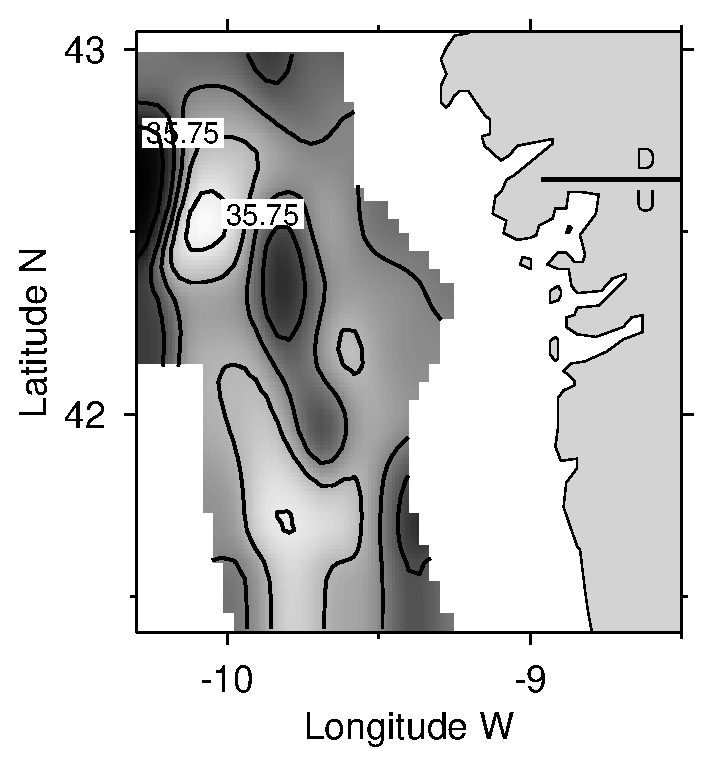
\includegraphics[trim=0 0 0 -15,clip,width=5.3cm]{cd105sal_200}}%
\subfigure[] {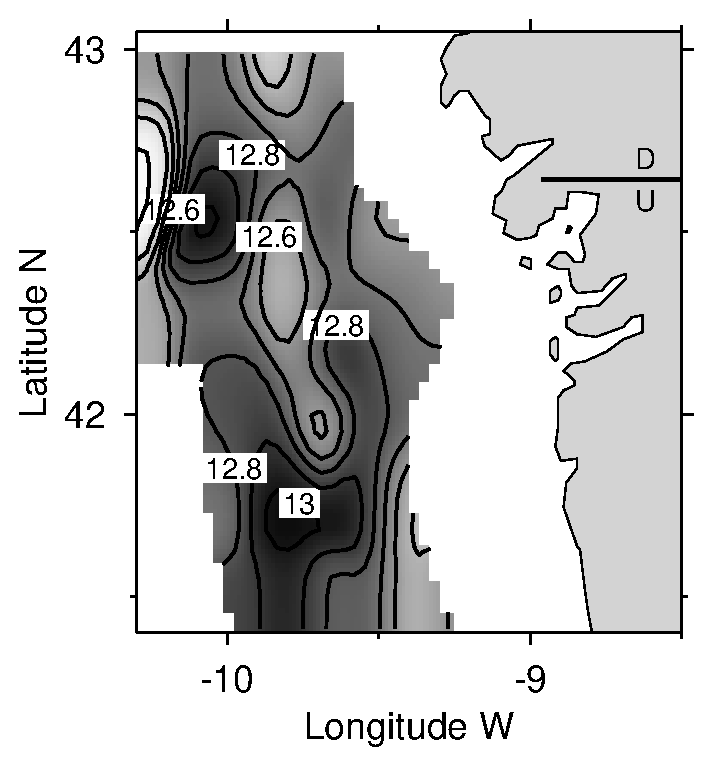
\includegraphics[trim=0 0 0
-15,clip,width=5.3cm]{cd105tem_200}} \subfigure[]
{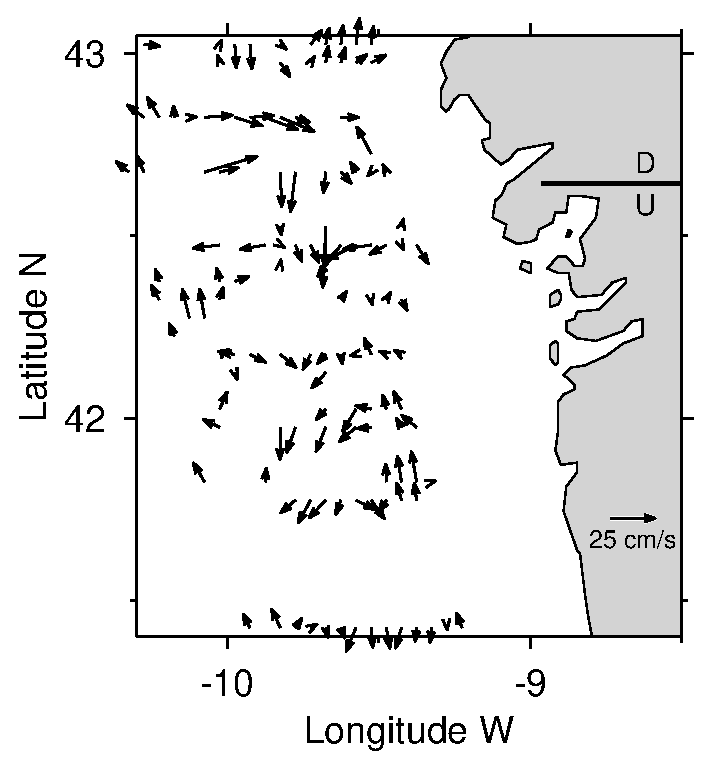
\includegraphics[width=5.3cm]{cd105adcpraw_191}}
\caption{Sub-surface (200m) properties during Leg B 10-20 June
1997. (a) Salinity; darker shading corresponds to lower salinity.
(b) Temperature; darker shading correspond to warmer temperatures.
(c) vectorised ADCP data with minimum averaging of 10min and 12m
in the vertical centred at 195m.The line on land indicates the
area sampled under upwelling (U) and downwelling (D) conditions.}
\label{fig:cd105_200m}\end{widefig}
\end{figure}

The non-divergent current field at 100m was similar but less
energetic than at shallower depths (Fig~\ref{fig:cd105_100m}c).
The offshore poleward flow, the northern coastal poleward current
and the anticyclonic eddy were all present down to 150m
(Fig~\ref{fig:cd105_150m}c), at which depth the coastal
equatorward flow had disappeared. The offshore flow off the Rias
Bajas at 42.25\deg N weakened with depth and disappeared below
150m. The meridional low salinity/temperature band clearly visible
at 100m can be traced as a southward flowing jet down to the
maximum penetration of the ADCP (Fig~\ref{fig:cd105_200m}c), at
which level a weakened poleward flow was still present offshore.

\FloatBarrier
\subsection{Vertical Fields}
\begin{figure}[!th]
\centering \subfigure[]
{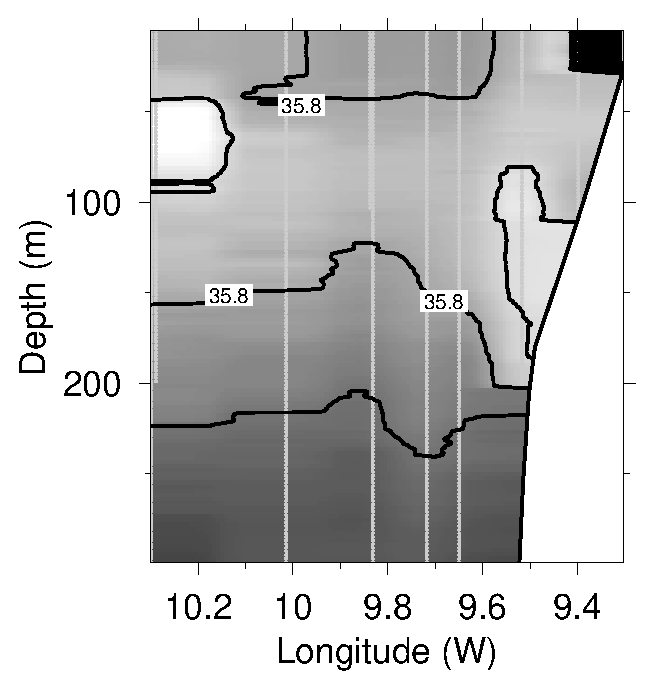
\includegraphics[trim=0 10 0 0,height=6cm,clip]{sectionN_S}}%
\subfigure[] {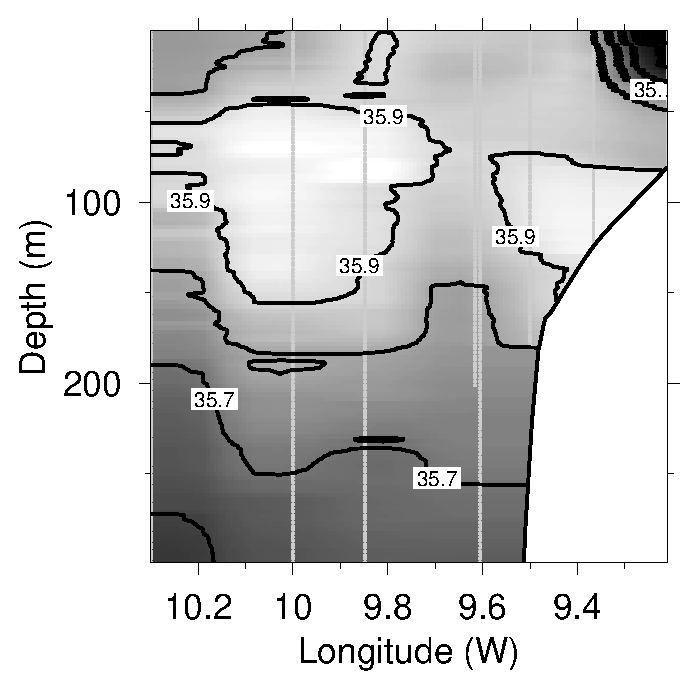
\includegraphics[trim=0 10 0
0,height=6cm,clip]{sectionP_S}} \subfigure[]
{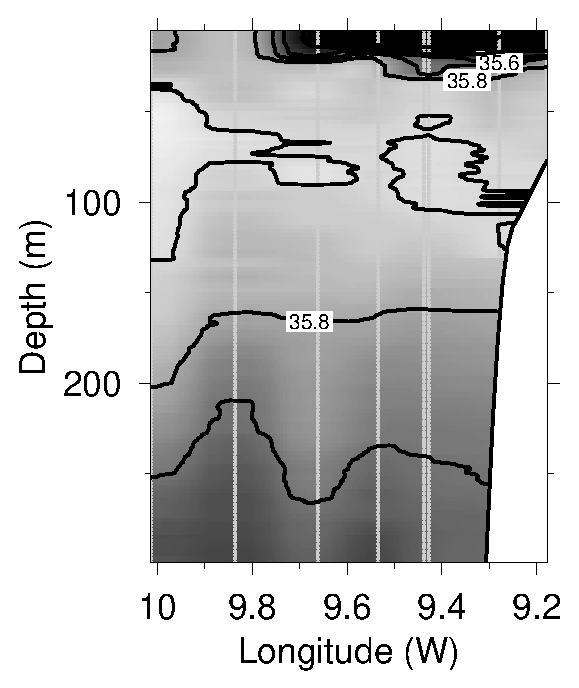
\includegraphics[trim=0 10 0 0,height=6cm,clip]{sectionQ_S}}
\subfigure[] {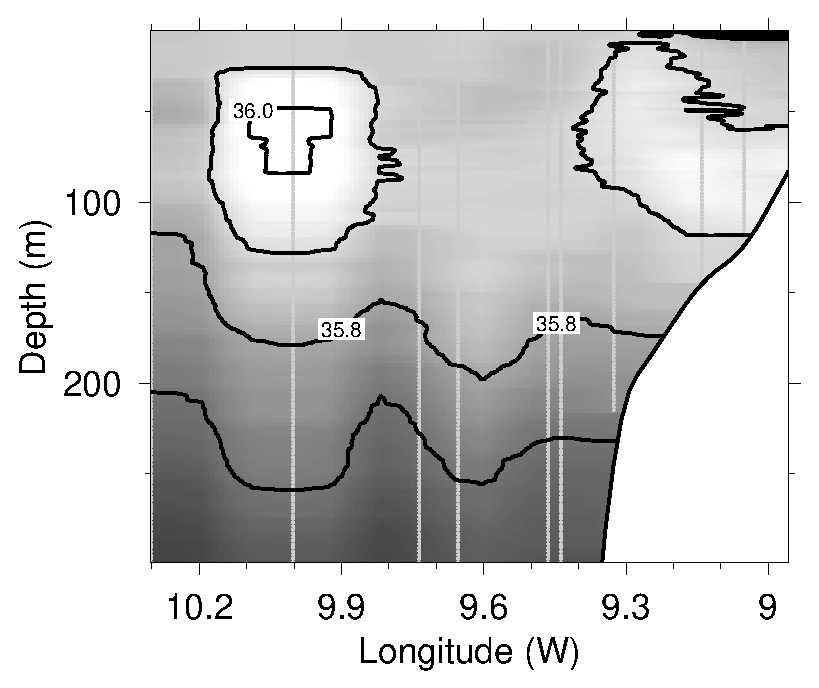
\includegraphics[trim=0 10 0
0,height=6cm,clip]{sectionS_S}} \subfigure[]
{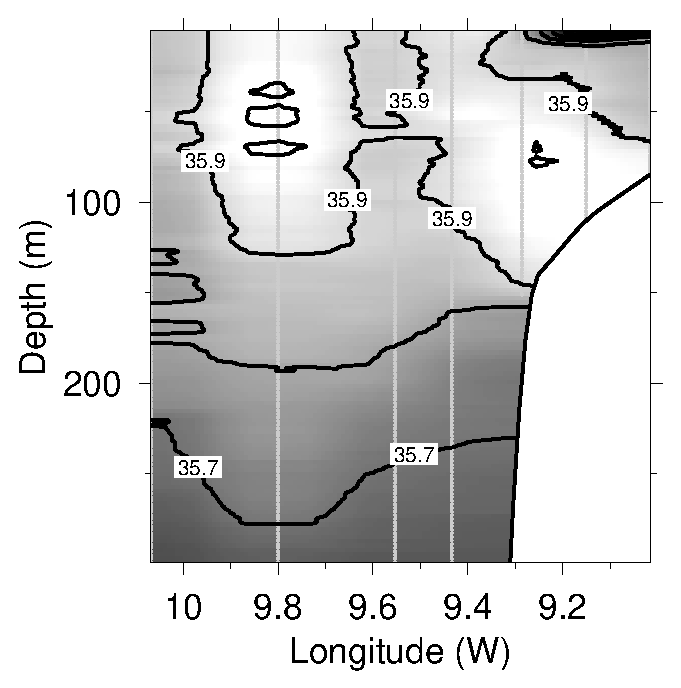
\includegraphics[trim=0 10 0 0,height=6cm,clip]{sectionU_S}}
\subfigure[] {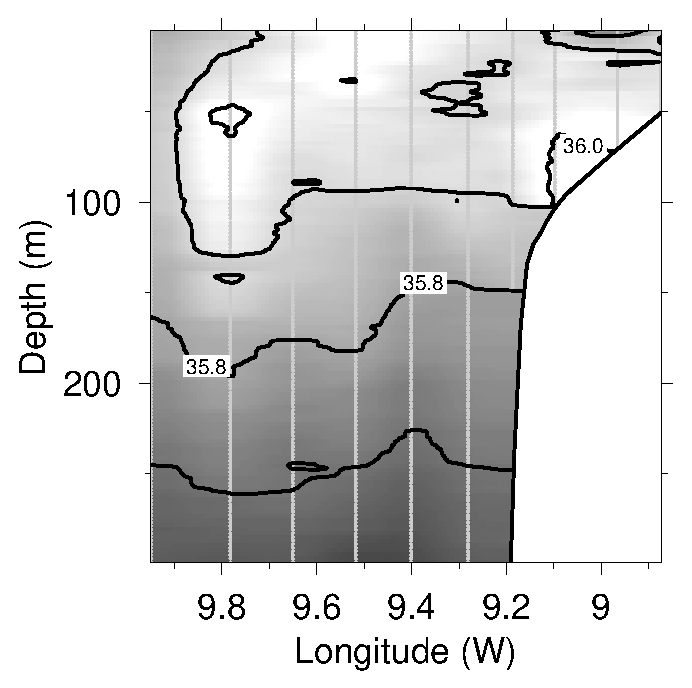
\includegraphics[trim=0 10 0
0,height=6cm,clip]{sectionV_S}}\caption{Vertical sections of
salinity for transects (a) N, (b) P, (c) Q, (d) S, (e) U and (f)
(V) down to 300m. Contouring interval is 0.1psu. }
\label{fig:cd105_sec_S}\end{figure}
\subsubsection{Salinity structure}
The top 300m of the salinity salinity structure is shown in
Fig~\ref{fig:cd105_sec_S} for transects (a) N, (b) P, (c) Q, (d)
S, (e) U and (f) V (locations in Fig~\ref{fig:cd105stations}). Two
maximum salinity cores ($>$35.9psu) can be seen in the range
50-150m at both the shelf and offshore and are associated with the
poleward flow seen in the surface contours. The offshore core is
consistently shallower and with higher values than the shelf core
but no clear meridional differences are apparent. The southernmost
section, transect V (Fig~\ref{fig:cd105_sec_S}f), shows three high
salinity cores; two of them at 50-100m, one on the shelf and one
offshore, and a shallower one 0-50m between the two. Although
their maximum values are located at surface to mid-depth, they can
still be seen at 300m, with local high salinities measured below
the salinity cores; the isohaline 35.8 in transect V deepens below
both the shallow and mid-depth salinity cores. At this latitude,
below 150m, the isohalines seem to have a positive slope, rising
shorewards.

As we progress northwards, the two sub-surface cores separate, and
maximum salinity in the cores decreases. In transect U, the
surface salinity maximum has disappeared, and the shelf branch has
deepened slightly. The 35.9 isohaline can be taken to represent
the core of the salinity maxima. In transect U, the 35.9 isohaline
has split into two cores, in contrast with transect V, and extends
to the surface from as deep as 150m over the shelf. A single
depression in deeper isohalines 35.8-35.7 can be seen under the
offshore salinity core, however, it is possible that the secondary
depression seen in transect V still exists at this latitude but
was not resolved by the sampling grid. A weak positive slope was
again measured at 150-200m associated with the 35.8 isohaline,
although the sign of the slope changes with depth as can be seen
in the 35.7 isohaline. Nearshore, on the shelf, a thin (15m)
surface layer of low salinity ($<$35.2psu) can be seen.

Further north, in transect S (Fig~\ref{fig:cd105_sec_S}d) the two
cores have reached their maximum separation (0.9\deg longitude).
Neither extends to the surface, and the shelf one has lower
salinity when compare to southern transects. The secondary
depression in the 35.7-35.8 isohaline seen in transect V,
separates the two salinity cores and is narrower than the one
under the offshore core but of similar vertical extension
($\thicksim$50m the displacement of the isohalines is similar). In
this occasion, the deeper isohalines show an overall negative
slope deepening shorewards. A thinner (10m) surface layer of low
salinity is present nearshore.

Transect Q (Fig~\ref{fig:cd105_sec_S}c) is located at the same
latitude as the Rias Bajas, and had the largest influence from
their freshwater outflow. A surface layer 25m thick of low
salinity ($35.8-35.5$psu) can be seen extending offshore, below
which the shelf high salinity core reaches a minimum in both
magnitude and dimension. The transect did not reached the offshore
limit of the poleward flow, but the offshore vertical structure is
very similar to transect S. The offshore salinity core limited by
the 35.9psu isohaline occupied a similar depth range than in
transect S, although peak salinity was lower. Below it, the local
deepening of the 35.7-35.8psu isohalines is of similar order to
transect S. However, the secondary depression is absent from the
35.8 isohaline but present again deeper in the 35.7 isohaline.

Transect P (Fig~\ref{fig:cd105_sec_S}b) showed the broadest and
deepest offshore salinity core (50-150m), and coincides with the
location of the anticyclonic eddy. There is still a low salinity
surface layer, deeper, reaching 50m, but more restricted to the
shore stations, extending only 20km offshore. The shelf salinity
core although less defined than at transect V,U and Q is
nonetheless more clear than in transect S. The salinity depression
separating the two cores is less well defined maybe as a result of
their proximity to each other. While the 35.7 isohaline still
experienced a weak local deepening between the two cores, the 35.8
isohaline instead showed an uplifting of 30m.

The northernmost transect, (N, Fig~\ref{fig:cd105_sec_S}a), had
the least proportion of high salinity core as determined by the
35.9psu isohaline. The offshore core was present only in the
50-100m range and the associated depression was less marked than
further south. The shelf core was situated at a deeper level,
reaching 180m and the 35.8psu isohaline deepened accordingly
shorewards, dropping 70m. Low salinity water was sampled in the
station closest to shore and a band of relatively low salinity
($<35.8$psu) can be seen in the top 50m between the high salinity
cores.

\begin{figure}[!th]
\centering \subfigure[]
{\includegraphics[trim=0 40 5 0,height=4.9cm,clip]{sectionNV}}%
\subfigure[] {\includegraphics[trim=0 40 5
0,height=4.9cm,clip]{sectionPV}} \subfigure[]
{\includegraphics[trim=0 40 10 0,height=4.9cm,clip]{sectionQV}}
\subfigure[] {\includegraphics[trim=0 40 10
0,height=4.9cm,clip]{sectionSV}} \subfigure[]
{\includegraphics[trim=0 40 5 0,height=4.9cm,clip]{sectionUV}}
\subfigure[] {\includegraphics[trim=0 40 5
0,height=4.9cm,clip]{sectionVV}}\caption{Vertical sections of
velocity component V for transects (a) N, (b) P, (c) Q, (d) S, (e)
U and (f) (V) down to 200m. Shading correspond to northward flow.
The 0 velocity contour appears as a dash line.}
\label{fig:cd105_sec_V}\end{figure}
\subsubsection{V component structure}
In general poleward flow was associated with the offshore limit of
the high salinity cores. Between the two salinity cores,
equatorward flow was measured at all depths as a relatively narrow
band. Poleward flow was also measured on the shelf edge on most of
the transects except for transect Q.

The southernmost transect, V (Fig~\ref{fig:cd105_sec_V}f), shows
good agreement with the salinity distribution, the offshore limit
of the salinity core being related to northward flow. The shift in
the salinity maxima seen between 9.6\deg-9.8\deg W has its
equivalent in the V component of the velocity, with northward flow
on its offshore limit($\thicksim$5\velc), and southward flow on
its onshore side. The latter, was consistently larger, 10\velc.

Transect U (Fig~\ref{fig:cd105_sec_V}e) had the same velocity
structure as in transect V, with northward flow on the offshore
side of both salinity cores (offshore and shelf edge) and
southward flow in between. The northward flow on the shelf reached
peak velocity between 25-50m (10-15\velc), decreasing with depth
until 100m after which values increased again. Maximum velocity in
the offshore branch occurred between 100-200m with similar values
to the shelf branch. The southward flow showed a core of maximum
velocity reaching values of 10-15\velc\, at 20-70m and decreased
with depth to 5\velc.

Transect S (Fig~\ref{fig:cd105_sec_V}d) shows again a similar
vertical structure, with surface intensified northward flow over
the shelf edge down to 50m (5\velc), and northward flow over the
entire column at the westward end. Again, the same relationship
with the salinity distribution holds, northward flow at the
offshore side of the salinity cores. In this case, the offshore
northward flow is not intensified at depth but in the top 50m
(10-15\velc). The southward flow between the two branches is again
surface intensified in the top 50m reaching values of 15\velc.
Nearshore, southward flow of 10\velc\, was measured and occupied
the entire water column.

The ADCP transect Q (Fig~\ref{fig:cd105_sec_V}c), reached further
offshore than the CTD transect Q, and sampled the offshore limit
of the salinity core. This time, no northward flow was measured
over the shelf edge, instead, southward flow occupied the entire
shelf, surface intensified and reaching values of 20\velc. The
southward flow found in all the transects reached here its highest
values over the entire water column (15\velc\,) as a narrow jet.
The offshore northward flow also had at this latitude the largest
values integrated over the entire water column (10\velc).

Transect P (Fig~\ref{fig:cd105_sec_V}b), which ran across the
anticyclonic eddy, had again the same basic structure with
northward flow over the shelf and offshore, and southward flow in
between. Both northward flows were surface intensified down to 80m
with values of 15\velc, while the narrow southward jet reached
peak velocities at 100-200m (15\velc).

The northernmost limit of the sampled region, transect N
(Fig~\ref{fig:cd105_sec_V}a), had the weakest (5\velc) and
narrowest southward jet. The main feature is a strong baroclinic
northward jet with values of 35\velc\, in the top 50m and
decreasing rapidly to 5\velc\, at 200m. The offshore northward
flow is weaker with average velocity of 5\velc\, throughout the
water column except for small intensification in the range 20-50m
at the westward end.

\begin{figure}[!th]
\centering \subfigure[]
{\includegraphics[trim=0 10 0 0,height=6cm,clip]{sectionN_T}}%
\subfigure[] {\includegraphics[trim=0 10 0
0,height=6cm,clip]{sectionP_T}} \subfigure[]
{\includegraphics[trim=0 10 0 0,height=6cm,clip]{sectionQ_T}}
\subfigure[] {\includegraphics[trim=0 10 0
0,height=6cm,clip]{sectionS_T}} \subfigure[]
{\includegraphics[trim=0 10 0 0,height=6cm,clip]{sectionU_T}}
\subfigure[] {\includegraphics[trim=0 10 0
0,height=6cm,clip]{sectionV_T}}\caption{Vertical sections of
temperature for transects (a) N, (b) P, (c) Q, (d) S, (e) U and
(f) (V) down to 300m.} \label{fig:cd105_sec_T}\end{figure}
\subsubsection{Temperature structure}
The temperature vertical structure is shown in
Fig~\ref{fig:cd105_sec_T} for the same transects as before. On
average, the thermocline was centred at 50m deepening at the
stations closest to shore, and rising locally over the sub-surface
salinity cores seen in Fig~\ref{fig:cd105_sec_S} and deepening
below. In the southernmost transects, V and U
(Fig~\ref{fig:cd105_sec_T}f-e) there is good correspondence
between the salinity distribution and the temperature structure.
The high salinity cores were locally related with higher
temperatures and deepening of the isotherms both on the shelf and
offshore where it reached below 300m. On the shelf edge, below
200m, the isotherms rose rather than sank in a similar way to the
salinity distribution. In the U transect
(Fig~\ref{fig:cd105_sec_T}e), the separation between the 14\deg
and 15\deg C isotherms in the shelf edge was larger than in
transect V, in response to the larger salinity core. Nearshore, in
the top 10-15m, the temperature increased to 19\deg C where
freshwater was encountered.

Further north, in transect S (Fig~\ref{fig:cd105_sec_T}d) the
general slope of the isotherms changes sign with respect to the
southern transects, becoming negative. The salinity cores produced
the same stretching in the temperature structure, which was more
pronounced offshore (75m, 10\deg W), than on the shelf (100m,
9.1\deg W). Similarly, the second salinity depression seen in
Fig~\ref{fig:cd105_sec_S}d below 150m at 9.6\deg W, is also
present in the temperature distribution.

The main difference found in transect Q
(Fig~\ref{fig:cd105_sec_T}c) with respect to other transects is
the uplifting of the isotherms eastward of 9.3\deg W in the top
50m. The surface layer (25m) of freshwater runoff from the Rias
also have a temperature signal, with values larger than 18\deg C.

Transects P and N (Fig~\ref{fig:cd105_sec_T}b-a) have in common
the marked deepening of the thermocline towards the shore down to
100m, in particular transect N. It has a marked effect in the
velocity field, where the largest horizontal shears in the
northward component were measured (Fig~\ref{fig:cd105_sec_V}a).

\begin{figure}[!th]
\centering \subfigure[]
{\includegraphics[trim=0 10 0 0,height=6cm,clip]{sectionN_D}}%
\subfigure[] {\includegraphics[trim=0 10 0
0,height=6cm,clip]{sectionP_D}} \subfigure[]
{\includegraphics[trim=0 10 0 0,height=6cm,clip]{sectionQ_D}}
\subfigure[] {\includegraphics[trim=0 10 0
0,height=6cm,clip]{sectionS_D}} \subfigure[]
{\includegraphics[trim=0 10 0 0,height=6cm,clip]{sectionU_D}}
\subfigure[] {\includegraphics[trim=0 10 0
0,height=6cm,clip]{sectionV_D}}\caption{Vertical sections of
density for transects (a) N, (b) P, (c) Q, (d) S, (e) U and (f)
(V) down to 300m.} \label{fig:cd105_sec_D}\end{figure}
\subsubsection{Density structure}
The density distribution was mainly determined by the temperature
structure. The pycnocline was centred at 50m overall, and it was
broader at the southern end of the grid (50m) than at the northern
end (30m). In most of the sections the pycnocline had a negative
slope nearshore except in transect Q (Fig~\ref{fig:cd105_sec_T}c),
where isopycnals as deep as 60m lifted. Surface stratification was
present in all transects, but was prominent in section Q, where it
reached furthest offshore.

The northward velocity component field showed qualitatively good
agreement with the density structure at large scales. Some of the
discrepancies between the velocity and density field could come
from the different resolution of the samplings. The downward
sloping of the isopycnals over the shelf edge corresponds to a
negative lateral density gradient which translates to a positive
geostrophic shear by the thermal wind equation, hence northward
flow against the sloping bottom (e.g
Fig~\ref{fig:cd105_sec_D}-~\ref{fig:cd105_sec_V}-b). In a similar
way, negative geostrophic shear, (equatorward flow) would be
related to positive lateral density gradient as in
Fig~\ref{fig:cd105_sec_D}b (100-200m; 10\deg-9.6\deg W), and when
this is not the case, forces other than Coriolis and pressure are
needed for dynamical balance, which is not surprising as we have
seen that the sampling took place during a transitional period.
\subsubsection{Assessing the variability during CD105}
\begin{table}[h]
  \centering
\begin{tabular}{ccccc}
\hline \hline \multicolumn{5}{c}{Data for the reference CTD} \\
\cline{1-5} CTD cast n\deg&Day&Latitude N&Longitude W&Cast depth\\
1&10 14:24& 42.6742&- 9.57720& 751.0\\
29&13 08:44& 42.6672&- 9.50000& 179.0\\
31&13 12:22& 42.6631&- 9.61580& 201.0\\
92&20 12:21& 42.6683&- 9.49440& 167.0\\
93&20 13:50& 42.6664&- 9.55220&487.0\\
94&20 15:04& 42.6658&- 9.60190& 985.0\\
\hline \hline
\end{tabular}
\caption{Time and location of CTD casts 1, 29, 31, 92, 93 and 94}
\label{tb:ctdref}
\end{table}

In order to investigate the effect of the wind shift during the
cruise in the hydrography of the region, 3 CTD cast pairs
(Table~\ref{tb:ctdref}) were selected from transect P at adjacent
positions, prior to and after the change in wind regime. The solid
lines in Fig~\ref{fig:refctd} correspond to casts before the
change in wind for both temperature (red) and salinity (blue).
Most of the variability is restricted to the top 75m, above the
thermocline. The three casts show the same changes, the surface
salinity dropped by $\thicksim 0.2$psu and surface temperature
increased by $\thicksim 0.7$\deg\, in response to the change from
southerly to northerly winds. The first CTD pair
(Fig~\ref{fig:refctd}a) corresponds to the first and last CTD
taken during the cruise and shows  differences similar to the
other two pairs, where the ``early'' CTD was taken on the last day
of southerly winds, 13 June. Hence, most of the change took place
after the wind shift.

The changes measured by the ADCP (Fig~\ref{fig:refadcp}) are less
straightforward to explain as the velocity field responds not only
to winds, tides and other oscillatory phenomena (i.e. inertial
waves, coastal trapped waves), but results from the interaction of
the offshore eddy and the advection of the freshwater plume off
the Rias Bajas as shown previously. The profiles in
Fig~\ref{fig:refadcp}a correspond to 40min averages centred at the
time of CTD 1 and 94 (Fig~\ref{fig:refctd}a). The standard
deviation in all profiles was consistently $\leqq 5$\velc. They
show a change from poleward flow (20\velc\, at the surface) with
constant negative vertical shear to a situation where the top 50m
reversed to equatorward flow of similar magnitude while the rest
of the water column flowed poleward with a smaller negative
vertical shear. The largest differences in the U-component took
place below the thermocline (50m), while the top 25m remained
unchanged. Below 50m, the flow changed from offshore before the
wind shift to onshore afterwards. Similar changes in the
U-component can be seen in the other profiles
(Fig~\ref{fig:refadcp}b-c), except that the change took place in
the top 75m rather than at the deeper levels where the flow was
close to zero. The northward component was not different from zero
in Fig~\ref{fig:refadcp}b while in \ref{fig:refadcp}c the flow
changed from equatorward to poleward below 50m, remaining
equatorward in the upper 50m.

\begin{figure}[!p]
\centering \subfigure[]
{\includegraphics[height=6cm]{ctdref1-94}}%
\subfigure[] {\includegraphics[height=6cm]{ctdref29-92}}
\subfigure[] {\includegraphics[height=6cm]{ctdref31-93}}
\caption{Vertical profiles of temperature (red) and salinity
(blue) for CTD casts (a) 1 (solid line) and 94 (dashed line), (b)
29 (solid) and 92 (dashed) and (c) 31 (solid) and 93 (dashed) down
to 200m.} \label{fig:refctd}\end{figure}
\begin{figure}[!p]
\centering \subfigure[] {\includegraphics[height=6cm]{adcpref1-94}}%
\subfigure[] {\includegraphics[height=6cm]{adcpref29-92}}
\subfigure[] {\includegraphics[height=6cm]{adcpref31-93}}
\caption{Vertical 40min averaged profiles of U (red) and V (blue)
components centred around the CTD casts (a) 1 (solid line) and 94
(dashed line), (b) 29 (solid) and 92 (dashed) and (c) 31 (solid)
and 93 (dashed) down to 200m.} \label{fig:refadcp}\end{figure}

\begin{figure}[!t]
\centering \subfigure[]
{\includegraphics[height=5cm]{vigoport_ths}}\\
\subfigure[] {\includegraphics[height=5cm]{vigoport_adcp}}
\subfigure[] {\includegraphics[height=5cm]{vigoport_st}}
\caption{Underway data collected at the start (10 June
08:45-10:31, red) and end (20 June 08:13-10:38, blue) of leg B of
CD105 cruise;  (a) temperature (solid line) and salinity (dashed
line), (b) top 50m ADCP vector currents with scale on the y axis
and (c) position of observations.} \label{fig:refths}\end{figure}

Changes are more dramatic nearshore when comparing underway data
(temperature, salinity and ADCP vector currents) from before and
after the wind shift. Two short sections are compared in
Fig~\ref{fig:refths} when the ship was leaving the port of Vigo
following a similar path at roughly the same velocity (4.5\vel).
Errors induced by the uncertainty in the ADCP calibration can be
assumed to be comparable during the two lines.

The surface values (Fig~\ref{fig:refths}a) showed a temperature
increase of over a degree centigrade, the disappearance of the
zonal temperature gradient and a reduction of 0.4psu in the
salinity west of 9\deg W after the onset of northerly winds. The
changes are larger than the ones measured in the reference CTDs,
as expected from the closer proximity to shore in this instance. A
narrow tongue of low salinity/high temperature was measured east
of 9\deg W on the 20 June and it likely originated from the Ria de
Arousa. A similar temperature and salinity distribution was
already encountered on the 18 June when the same region was
occupied for the first time after the wind shift of the 14 June.

The flow in the top 50m (Fig~\ref{fig:refths}b) was northward
($\thicksim 20$\velc) at the time of the first line and followed
roughly the orientation of the coast.At the end of cruise, the
flow reversed after the wind shift, maintaining a similar
orientation and reached a peak velocity of $\thicksim 35$\velc.
Both flows had a narrow jet geometry with similar zonal scales.
The low salinity tongue was probably advected southwards rather
than offshore by the southward coastal jet measured at the time.

\subsection{Water mass analysis}
\begin{figure}[t]
\centering \begin{minipage}{7cm} \subfigure[]
{\includegraphics[width=7cm]{tsplot}}%
\end{minipage}
\begin{minipage}{4cm}
\subfigure[] {\includegraphics[width=4cm]{tsplot_st}} \subfigure[]
{\includegraphics[width=4cm]{tsplot_small}}
\end{minipage}\caption{T/S characteristics found during CD105 for
selected CTD casts. (a) T/S diagram down to a maximum depth of
1800m for the colour coded sub-regions, (b) CTD casts position and
(c) blow up of the T/S diagram. All share the same colour codes. }
\label{fig:cd105ts}\end{figure}

The typical water mass distribution explained in
Chapter~\ref{ch:litrev} was well represented in CD105 cruise. The
upper waters of the Iberian coastal ocean were divided into a
surface mixed layer above a seasonal thermocline reaching down to
100m, and then the permanent thermocline, down to 500m, where the
influence of the Mediterranean outflow began. The permanent
thermocline had the characteristic linear relationship between
temperature and salinity typical of Eastern North Atlantic Waters
(\enaw).

From the CTDs collected during the cruise 6 sub-regions have been
defined to investigate the T/S differences among them
(Fig~\ref{fig:cd105ts}). The graph shows the subdivisions of the
\enaw as \enawt and \enawp, and their shared limit H defined by
\citet{Rios92}. The 6 sub-regions correspond to latitudinal and
zonal variations in relation to the poleward flow and the regions
of influence of the Rias Bajas and the Mi\~no river. Their
influence can be seen in the top 10-25m for the regions labelled
Southward Coastal Jet (SCJ) and Minho runoff (M) (see
Fig~\ref{fig:cd105ts}b for their exact location). Their surface
salinity fell below 35psu at the stations nearer to shore, and
increased offshore.

The bulk of the central waters are \enawt, with only a small
portion lying on the \enawp line definition. As we move northward
(Fig~\ref{fig:cd105ts}c), the surface salinity decreases defining
a high salinity maximum at the level of the \enawt (100m) which
gradually reduces with latitude. The exception is the southward
coastal jet region, where the maximum is of similar value to the
North nearshore region suggesting the southward advection of
waters from the poleward flow.

Below the central waters we find the Mediterranean Water (MW) high
salinity core, which corresponds to the vein of MW flowing
northwards along the continental slope between 800-1300m. No
evidence was found of the two main outflow cores of MW normally
located offshore at $\approx$750 and $\approx$1250m
\citep{Zenk90}. The MW high salinity core reduced with latitude
and offshore in agreement with its northward advection along the
slope.

\section{Discussion}
In mid-latitude continental shelves the spring transition is
determined by the net surface heat flux as it changes from cooling
to warming \cite{He02}. Near the mouth of the Ria de Vigo, such
transition takes place in April as estimated from bi-weekly data
for the period 1987-1992 \citep{Nogueira97}. From November to
March, thermal inversion takes place, the water column becomes
briefly homogeneous in early April and remains stratified until
October, when thermal inversion develops once more. Similar trends
can be expected in the shelf, considering the strong linkage
between the Rias and the shelf \citep{Alvarez-Salgado00}. However,
the transition between the downwelling winter regime and the
upwelling summer regime typically takes place in June, two months
after the spring transition \citep{Nykjaer94}. The Charles Darwin
CD105 cruise took place during that transition from the winter
downwelling to the summer upwelling season, from 10 to 20 June.

\subsection{General circulation}
During Leg A, surface salinity hinted at the presence of a
contorted poleward current, the PCC. In the southernmost transect,
the PCC reached the slope, separated from it further north
(maximum opposite the Rias Bajas) and turned back to the slope
south of Cape Finisterre. The weekly SST average showed a similar
trend, with the high salinity tongue associated with warmer
temperatures. Scattered along the warm tongue were warm patches
suggestive of anticyclonic eddies. Their SST signal suggested a
spatial scale of $\sim$30-40km. Eddies associated with the PCC
have been previously reported \citep{Haynes91,Sena96}. Evidence of
the poleward flow SST signal separating from the slope between
41.5\deg-42\deg N are also present in May when some coastal
upwelling was also measured. The SST distribution is very similar
to Fig~\ref{fig:cd105sst}a and coincide with the absence of
poleward flow north of Cape Finisterre.

A similar picture arises from Leg B, except a southward jet was
present over the inner shelf in response to northerly winds. High
salinity values are the distinctive mark of the PCC. Previous
studies of the PCC in the west coast of Iberia (40\deg N) have
also found a high salinity core at 100m close to the slope
\citep{Frouin90,Haynes90}. The double core structure of the
salinity data is however surprising but could be related to strong
winter upwelling episodes and be only present towards the end of
the downwelling regime. Both the offshore subsurface salinity
maximum and poleward flow were better defined than the shelf edge
salinity maximum, particularly opposite the Rias Bajas. Those were
the transects sampled at the end of cruise, after the shift in
winds. However,similar differences were observed between both
salinity maxima in the northernmost transect sampled during strong
downwelling winds. The weaker salinity signal over the shelf edge
could then correspond to a more intermittent poleward flow branch
during the final stages of the downwelling regime reactivated in
the face of downwelling favourable winds. The offshore salinity
maximum coincided with northward velocities up to 15\velc\,
smaller than the average speed of 27\velc\, measured by
\citet{Haynes90} which reached depths of 400m in association with
the PCC. Smaller and more discontinue northward velocities were
associated with the shelf edge salinity maximum. Between the two
salinity maximum, southward flow was present in all transects at
all depths associated with a low salinity and temperature wedge.
It advected waters from north of Cape Finisterre as inferred from
SST images and its presence as early as May could indicate a
circulation feature of the end of the downwelling regime.

One offshore anticyclonic Eddy related to the PCC was evident in
the data. Its SST signal disappeared after the 6-8 June storm but
it was still present in the cruise data. It had an estimated
diameter of $\sim$30-40km from both surface SST and \emph{in situ}
data to a depth of 150m, carrying $\sim$128\vol. They are
different from SWODDIES which form in the Bay of Biscay
\citep{Pingree94} and have also been linked to the PCC. Their
characteristic radii can be four times bigger (50-60km) and reach
depths of 1500km. However, the present data are insufficient to
hypothesize about its life span or its origin. \citet{Huthnance02}
presented eddy statistics for a region 40.5-45.5\deg N out to
13\deg W for years 1993-1999. They had a mean diameter of $\sim
52\pm 22$ based on their SST signal and most were found north of
Cape Finisterre-Cape Ortegal a preferred eddy generation area
\citep{Dubert98,Paillet02}. Although they constitute an active
shelf exchange mechanism their small number (20 per year) makes a
modest contribution to the overall exchange in the region
\citep{Huthnance02}. A cyclonic eddy like re-circulation was
apparent on the shelf slightly south of 42\deg N but its velocity
signal was less well defined. It is located at a filament site
\citep{Haynes93} and might be related to the topography, as the
coast and shelf orientation changes, and the offshore shelf flow.

Coexistence of the PCC and coastal upwelling has been previously
reported \citep{Castro97,Peliz02}. The PCC reached its maximum
westward position opposite the Rias Bajas, and seaward flow was
measured there. The seaward flow was related with the low
salinity/ high fluorescence Rias outflow. The offshore extension
of the low salinity plume has values not less than 35.5, when we
could have expected lower values like further south off the
Mi\~{n}o mouth. It thus provides evidence that shelf waters get
piled up inside the Rias, mixed with riverine flow inside the
Rias, and when downwelling winds relax or change to northerly
winds the waters are flushed to the shelf. Also, where the Rias
Bajas break the coastline, the corresponding portion of upwelling
appears to occur within the Rias \citep{Alvarez-Salgado00} and
flushing is enhanced. The offshore extend of the freshwater plume
increases due to the enhanced stratification, suppression of
turbulence and response to Ekman across-shelf mass transport force
by local winds \citep{weisberg01}.

In summary, drastic changes occur in the inner shelf from both the
wind forcing and buoyancy input from the Rias. Inner shelf
circulation changes and the effect is progressively advected
offshore where it interacts and affects the shelf circulation.
Local winds are a major driver of the inner shelf circulation
\citep{weisberg01}, which in turn produces large changes in the
stratification through catastrophic release of Rias waters. The
jet structure of the flow in the inner shelf comes about from the
balance between the sloping topography, bottom friction and wind
forcing.


%Other possibility is the
%release of piled up water in the Rias when northward winds weaken.
%As the poleward flow moves offshore, it leaves space for an
%equatorward geostrophic flow to develop in response to the sloping
%isopycnals of the shoreward side of the poleward. Also, at some of
%the transects, particularly those in the middle of the grid, show
%a double relatively high salinity core at depths below 150-200m,
%which could represent the previous and present position of the
%poleward flow, that take longer to erode?.


\section{Conclusions}
Data from the transition between the downwelling and upwelling
regimes have been presented. The picture is one of complex
circulation, where slope poleward flow coexists with coastal
upwelling and strong Rias outflow. The interaction generates
eddies carrying PCC waters which could help in the disappearance
of the PCC during the start of the upwelling regime.
\begin{itemize}
\item Mesoscale activity during the spring transition is high.
The data showed eddies which interact with the PCC.
\item Two poleward flow branches exist, one at the slope which
is promoted in the absence of upwelling winds and an offshore one
that develops during episodes of upwelling winds.
\item The branching can be seen in SST originating near 41.5\deg
but the formation mechanism is not clear.
\item The two branches are more readily discernible at the end of
the downwelling regime.
\item The Rias do influence the circulation regime of the shelf,
possibly enhancing offshore flow.

\end{itemize}
